%%%%%%%%%%%%%%%%%%%%%%%%%%%%%%%%%%%%%%%%%%%%%%%%%%%%%%%%%%%%%%5
%% ITB Author: Markus Hofmann - markus.hofmann@itb.ie
%% Adapted from Dalhousie University
%% Used by Adam O'Connor
%% Language used
%% !TeX spellcheck = en_GB
%%%%%%%%%%%%%%%%%%%%%%%%%%%%%%%%%%%%%%%%%%%%%%%%%%%%%%%%%%%%%%%5


\documentclass[12pt,ITBthesis]{report}
\usepackage{textcomp}
\usepackage{amsfonts}
\usepackage{amssymb,amsmath}
\usepackage{amsthm}
\usepackage{newlfont}
\usepackage{graphicx}
\usepackage{tabularx}
\usepackage{longtable}
\usepackage{lscape}
\usepackage{booktabs}
\usepackage{latexsym}
\usepackage{natbib}
\usepackage{geometry}
\usepackage{fancyhdr}
\usepackage{xthesis}
\usepackage{xtocinc} %Include Table of Contents as the first entry in TOC
\usepackage{tabu}
\usepackage{subfigure}
\usepackage{times}
\usepackage[hidelinks]{hyperref}
\usepackage{listings}

\lstdefinestyle{myCustomMatlabStyle}{
	language=Java,
	stepnumber=1,
	numbersep=10pt,
	tabsize=4,
	showspaces=false,
	showstringspaces=false
}

\bibpunct[, ]{(}{)}{;}{a}{,}{,}


\begin{document}

%%% this section is responsible for creating bookmarks and cross-links in your pdf document
%\hypersetup{bookmarksnumbered=true, colorlinks=false, bookmarksopen = false, linkcolor=blue ,
%linkbordercolor = 3 3 3, citebordercolor = 3 3 3, urlbordercolor = 3 3 3}


% Fuzz -------------------------------------------------------------------
\hfuzz2pt % Don't bother to report over-full boxes if over-edge is < 2pt
% Line spacing -----------------------------------------------------------

\newlength{\defbaselineskip}
\setlength{\defbaselineskip}{\baselineskip}
\newcommand{\setlinespacing}[1]%
           {\setlength{\baselineskip}{#1 \defbaselineskip}}
\newcommand{\doublespacing}{\setlength{\baselineskip}%
                           {2.0 \defbaselineskip}}
\newcommand{\singlespacing}{\setlength{\baselineskip}{\defbaselineskip}}
% MATH -------------------------------------------------------------------
\newcommand{\A}{{\cal A}}
\newcommand{\h}{{\cal H}}
\newcommand{\s}{{\cal S}}
\newcommand{\W}{{\cal W}}
\newcommand{\BH}{\mathbf B(\cal H)}
\newcommand{\KH}{\cal  K(\cal H)}
\newcommand{\Real}{\mathbb R}
\newcommand{\Complex}{\mathbb C}
\newcommand{\Field}{\mathbb F}
\newcommand{\RPlus}{[0,\infty)}
%
\newcommand{\norm}[1]{\left\Vert#1\right\Vert}
\newcommand{\essnorm}[1]{\norm{#1}_{\text{\rm\normalshape ess}}}
\newcommand{\abs}[1]{\left\vert#1\right\vert}
\newcommand{\set}[1]{\left\{#1\right\}}
\newcommand{\seq}[1]{\left<#1\right>}
\newcommand{\eps}{\varepsilon}
\newcommand{\To}{\longrightarrow}
\newcommand{\RE}{\operatorname{Re}}
\newcommand{\IM}{\operatorname{Im}}
\newcommand{\Poly}{{\cal{P}}(E)}
\newcommand{\EssD}{{\cal{D}}}
% THEOREMS ---------------------------------------------------------------
\theoremstyle{plain}
\newtheorem{thm}{Theorem}[section]
\newtheorem{cor}[thm]{Corollary}
\newtheorem{lem}[thm]{Lemma}
\newtheorem{prop}[thm]{Proposition}
%
\theoremstyle{definition}
\newtheorem{defn}{Definition}[section]
%
\theoremstyle{remark}
\newtheorem{rem}{Remark}[section]
%
\numberwithin{equation}{section}
\renewcommand{\theequation}{\thesection.\arabic{equation}}
%%% ----------------------------------------------------------------------
\setlength{\tclineskip}{1.05\baselineskip}
%%% ----------------------------------------------------------------------
\makeatletter
\renewcommand\appendix{%
 \par
 \setcounter{chapter}{0}%
 \setcounter{section}{0}%
 \setcounter{subsection}{0}%
 \gdef\thesection{\@Alph\c@section}
 \gdef\@sect##1##2##3##4##5##6[##7]##8{%
  \refstepcounter{##1}%
  \protected@edef\@svsec{\@seccntformat{##1}\relax}%
  \begingroup
    \hspace{-\parindent}##6\appendixname~ {%
    \@hangfrom{\hskip ##3 \relax\@svsec}\par%
    \hspace{-\parindent}\interlinepenalty \@M ##8 \@@par}%
  \endgroup
  \csname ##1mark\endcsname{##7}%
  \addcontentsline{toc}{##1}{\protect\numberline{\csname the##1\endcsname}##7}%
  \@xsect{##5}%
 }%
}%
\makeatother

\setlength{\parskip}{1ex plus 0.5ex minus 0.2ex}


\title{INFORME@DUBLIN AN ANDROID APPLICATION THAT SHOW’S THE HISTORY OF DUBLIN AND SURROUNDING AREAS}

\author{Adam O'Connor }

\university{Institute of Technology Blanchardstown }

\dept{School of Informatics and Engineering }

\address{Dublin, Ireland }

\supervisor{Dr. Simon McLoughlin}

\submitdate{17 May 2017 }

\degree{BSc (Hons) in Computing }


%\dedicate{To my wife\\
% \begin{Huge}{\textbf{Glenda}}\end{Huge}}

%\nobib
%\draft
%\nofront
%\permissionfalse
%    % Thesis Abstract ------------------------------------------------------

\prefacesection{Abstract}

The project in hand takes on the role of a software developer which is a computer science student at the Institute of Technology Blanchardstown. The proposer of the project puts into focus, that historical monuments which are located throughout the suburb's and city of Dublin have been neglected over some time on which the developer wishes to change. Bringing the past and present together as one is what the application is trying to achieve as well as educating local people about their area.
\par
The proposer of the project is willing to design and implement a location-aware Android application which provides Geofence locations of specific historical monuments. On entering such a monument, the Information will then be presented to the user of such device. The language of which the app would be coded will be Java on which the developer has learned over numerous years.
\par
The following application would provide an inexpensive way of displaying historical information to patrons of the app and other tourists of which wish to learn about Dublin. The application could change the way locals and tourists learn about the surrounding area of Dublin. The developer will contact Dublin county council and Fingal county council to receive their feedback or funding for the rollout of such an application to the general public.

\smallskip


% ----------------------------------------------------------------------


\setcounter{page}{1} \beforepreface

{ \typeout{Abbreviations}
% Thesis Abbreviation ------------------------------------------------------

\prefacesection{Abbreviations}


%%%%%%%%%%%%%%%%%%%%%%%%%%%%%%%%%%%%%%%%%%%%%%%%%%%%%%%%%%%%%%%%%%%%%%%%%%%%%%%%
% Create a list of all abbreviations that you've used throughout your thesis.  %
% Order the abbreviations in alphabetical order                                %
%%%%%%%%%%%%%%%%%%%%%%%%%%%%%%%%%%%%%%%%%%%%%%%%%%%%%%%%%%%%%%%%%%%%%%%%%%%%%%%%

\begin{longtable}{p{90pt}l}
\hline APP      & Application \\
\hline OS     	& Operating System \\
\hline CSS 		& Cascading Style Sheet \\
\hline GNU      & GNU's Not Unix \\
\hline IDE      & Integrated development environment \\
\hline PaaS		& Platform as a Service \\
\hline IaaS     & Infrastructure as a Service \\
\hline LBS      & Location Based Services \\
\hline ADB      & Android Debug Bridge \\
\hline GCM       & Google Cloud Messaging \\
\hline WAH       & Windows Azure Hypervisor \\
\hline GPS       & Global Positioning System \\



\hline
\end{longtable}






% ----------------------------------------------------------------------
 %write your list of abbreviations in a file called abbreviations.tex
}


% ------------------------------------------------------------------------
\afterpreface
\def\baselinestretch{1}
\setlinespacing{1.66}
% ------------------------------------------------------------------------

\pagestyle{fancy}
\renewcommand{\chaptermark}[1]%
{\markboth{\MakeUppercase{\thechapter.\ #1}}{}}
\renewcommand{\sectionmark}[1]%
{\markright{\MakeUppercase{\thesection.\ #1}}}
\renewcommand{\headrulewidth}{0.5pt}
\renewcommand{\footrulewidth}{0pt}
\newcommand{\helv}
{%
\fontfamily{bch}\fontseries{b}\fontsize{9}{11}\selectfont} \fancyhf{} \fancyhead[LE,RO]{\helv \thepage}
\fancyhead[LO]{\helv \rightmark} \fancyhead[RE]{\helv \leftmark}
% ------------------------------------------------------------------------
\setlinespacing{1.0}

\chapter{Introduction}

\section{Background}
From the beginning of time finding information about particular areas or building was a kind of tricky job unless you knew where to go or whom to talk to about the history attached to these certain places. More recently we can access websites and see the information about a certain location or area. Usually, the Dublin county council office has the data on each town for example Lucan. With the suburbs growing steadily over the last number of years the changing of towns has been in an extraordinary state. Towns that have been around for hundreds of years are the main reason for the development of such an application (App) so that Dublin's history can be brought back to life.
\par
What the developer is willing to achieve is to allow people to navigate, explore and learn about the history of different buildings. Throughout the use of this application, the user's will then grasp a better knowledge of the area in which they live.
Throughout the development of the Android Operating System (OS) starting in 2006 steadily numbers grew after Google's release of sharing its operating system to all mobile manufacturer's. The first mobile to be released with such an OS was the HTC Dream.\cite{androidHtc}  which is why the developer has chosen to develop an android application.
With the introduction of the Google play market, which launched on the March 6th,  2012, There has been a huge demand for smart technology. Now we can use our mobile phone for doing just about anything, such as surfing the web, reading emails, even playing games and the interpretation of books. 


\section{Introduction of the InforMe@Dublin Project}

With regards to the following proposed project on which its aim is to provide additional information to tourists or just the common public who wish to learn more about the history of their local area and wish to view old photos or view historical places in their area. When the user is in this specific area pop-ups will appear that can be selected and information will then be display for that designated place. Users may post their findings of images whether that be past or present to allow others to learn from what users have posted.
\par
The information such as the history of the area will be sourced from a variety of on-line sources that will be compiled by the developer. The information will be accessed by the application using Firebase database which is a cloud storage service for Android, OS and web projects of which was created by Google.
\par
With the research that has been uncovered in the literature review of the following thesis. The developer has then chosen what technologies should be used in order to complete the InforMe@Dublin application.

\section{Research Question's}
The Research questions of which the developer must answer are defined below. Each of these questions will be answered throughout the following thesis.
\begin{enumerate}
	\item\textbf{\textit{Is there a need for an application like this on the marketplace?}}

	\item\textbf{\textit{Is there a way to save battery life while using GPS / Internet connection within an android application?}}

	\item\textbf{\textit{Will location services, and mobile internet take much battery or data?}} 

	\item\textbf{\textit{Will the APP provide a wiki type interface where visitors can add to the information about a historic site?}}
	
\end{enumerate}    






\chapter{Project Management}

\section{Project Name / Supervisor / Manager }    Project \hspace{2mm} \textemdash \hspace{2mm} InforMe@Dublin
\newline
Supervisor \hspace{2mm} \textemdash \hspace{2mm}  Dr Simon McLoughlin
\newline
Manager \hspace{2mm} \textemdash \hspace{2mm}  Adam O\textquotesingle Connor

\section{Success Criteria}
\begin{itemize}
	\item The complete program should be able to locate their current location and if a building of significant historical value.
	\item The program should allow other users to learn and about their area.
	\item The program also allows the users to explore their town and get fit by doing so.
	\item The application should educate the user and tell them the information.
	\item Program should have great user functionality and work very efficiently for the user.
	\item Should be very user-friendly.
\end{itemize}

\section{Assumptions Risks and Obstacles }
\begin{itemize}
	\item Coding a responsive application for the Android operating system.
	\item Using the Google Maps API and location service's that are incorporated into an android device.
	\item Using Android Studio to create this application.
	\item Coding from scratch and learning new technologies on the way.
	\item Allocating time and resources to develop the application as a whole.
	\item Timekeeping to allow us for the project to be completed within a reasonable time-scale.
\end{itemize}

\section{Motivation for choosing project}
With the influence of new mobile technologies throughout this day and age, the developer has always seen a niche market for an application that utilises and explores the user's town. Everyone has readily available internet connectivity on our mobile phones and if not a GPS module incorporated into that device. With towns growing rapidly throughout the years all the hidden gems of these area's are being left behind with no-one knowing the history of what is there.

A developers job is to either make things easier on people or to produce new idea's or technologies for a normal user to use. The only flaw of this project is the user needs to own an Android device and have an internet connection. The project enables the user to walk around their town and to discover new areas with the use of this app. The app should provide some Wikipedia type adjustments that will be sent to the admin or requests to show lost monuments or where historical relics have been found.

Due to some of the historical finds that have been found around Dublin and some of the structures with the likes of Neolithic axes found as well as the oldest bridge in Ireland that provides passage over the Griffeen Valley River.

\newpage

\section{Methodology}
\textbf{V Model}
The model that we will be using to develop this project will be the V – Model, why the developer chose this model, is because the steps in progress are in a sequential manner in and the type in question is also known as the verification and validation model. Which means after each step is complete, the software and hardware are both Verified and validated.
The model chosen is an augmentation of the waterfall model and is based on the testing of each phase of the development which means each step of the development life-cycle there is then a directly associated testing phase with each part of code. The type of proposed model, as follows, is a highly disciplined model in that the next step only starts on completion of the open phase.
\cite{TPoint}


\begin{figure}[htbp]
	\center 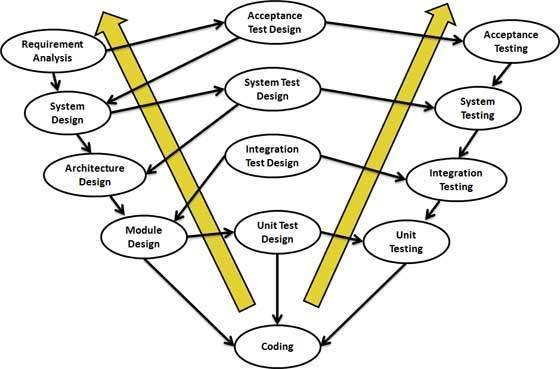
\includegraphics[width=400pt]{vshapedmodel}\\
	\caption{Image of the V Model \citep{TPoint}} \label{Figure: V Shaped Model 
		Area}
\end{figure}

\newpage
\begin{table}[!ht]
	\section{Work Breakdown Structure}
	\begin{tabular}{ l l l }
		\textbf{Objective} && \textbf{Task} \\
		Complete Project Proposal. && Complete within 2 weeks. \\
		Research and test Google maps API and geo-location. && Complete within 1 week. \\
		Research android application development with the cloud. && Complete within 1 week. \\
		Preform literature review on the project. && Complete within 2 weeks. \\
		Risk analysis. && Complete within 2 weeks. \\
		Development plan. && Complete within 1 week. \\
		Build prototype. && Complete within 3 weeks. \\
		Second risk analysis. && Complete within 1 week. \\
		1st validation and verification. && Complete within 1 week. \\
		Operational prototype. && Complete within 1 week. \\
		2nd validation and verification. && Complete within 1 week. \\
		Final development. && Complete within 2 weeks. \\
		Implementation. && Complete within 1 week. \\
	\end{tabular}
	\caption{Table of Work Breakdown Structure.}
	\label{table : Work Breakdown Structure.}
	\newpage
\end{table}

\section{Technologies and Skills Needed}
\begin{enumerate}
	\item Programming  in the Java development language.
	\item Using and incorporating APIs into Android applications.
	\item Knowledge of XML for design layouts.
	\item Knowledge of JSON.
	\item Knowledge of Firebase and its associated methods.
	\item Experience of using Google's developer console.
	\item Experience of developing application's for Android devices.
	\item Using and adapting gradle properties of Android applications.
	\item Underlying architecture of the Android OS.
	\item Utilising modules of the Android Device.
	\item Learning new permission requests of Android Marshmallow and above.
	\item Utilising the battery life of Android devices.
	\item Knowledge of Location Services.
	\item Knowledge of Computational processes of Android devices.
\end{enumerate}

\section{Gantt Chart}
Below is a following gantt chart with regards to the work of which will be completed by the developer throughout the development of such an application of this size.
\begin{figure}[!ht]
	\center 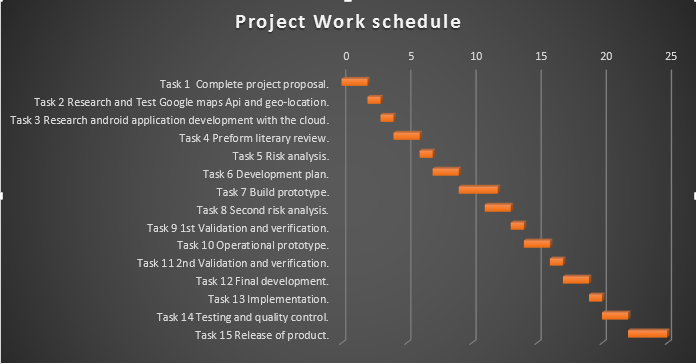
\includegraphics[width=420pt, height=250pt]{ganntChart}\\
	\caption{Gantt Chart} \label{Figure: Gantt Chart of work breakdown structure.  
		Area}
\end{figure}

\newpage

\section{Development Device}
Concerning the development section of the following thesis of which is about the device on which the Android application would be developed on. The device in question is as follows -

\begin{table}[!ht]
	\begin{tabular}{ l l l }
		\textit{Mobile Name} && Alcatel Pop 4+ \\
		\textit{Operating System} && Android 6.0 (Marshmallow)\\
		\textit{CPU} && Quad-core 1.1 GHz Cortex-A7 \\
		\textit{Chipset} && Qualcomm MSM8909 Snapdragon 210 \\
		\textit{RAM} && 1.5GB Ram \\
		\textit{Internal Memory} && 16GB \\
		\textit{Battery} && Removable Li-Ion 2500 mAh battery \\
	\end{tabular}
\caption{Alcatel Pop 4+ Specifications.}
\label{table : Alcatel Pop 4+ Specifications.}
\end{table}

\begin{figure}[!ht]
	\center 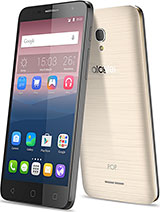
\includegraphics[width=150pt, height=250pt]{alcatel}\\
	\caption{Alcatel Pop 4+} \label{Figure: Alcatel Pop 4+}
\end{figure}

\newpage
\section{Conclusion}
This project as a whole is ready to start. Some changes may occur during the development throughout the build and production. The next stage of the project in the question is to research all available sources and technologies that can be used in the creation of such project. The Finished development of the application scheduled for the end of April 2017, with a mock-up build of the project due in December 2016.

\chapter{Literature Review}

\section{The New Era of Mobile Phone Technology}
Regarding the mobile phone industry first starting off and then rapidly building over the past 49 years when the first cell phone that was produced by the Motorola company. That makes the very first hand-held modular phone created on the 3rd of April 1973, By Martin Cooper, he was also a Motorola researcher and executive who developed the only type of hand-held subscriber equipment. Martin placed the first call to Doctor Joel S. Engel of Bell Labs.
\newline
\newline
A funny side of this story was because Bell Labs and Motorola where in direct competition to develop this kind of technology. This mobile phone weighed 1.5 kilos on which the talk time was only 30 minutes and took 10 hours to charge its battery full. \cite{cellHist}
\newline
\newline
Compare this to a mobile phone device to today's standards. The Samsung Galaxy S7 edge which weighs a biscuit crumbling 157 grammes which also holds a large talk time of 27 hours and a full charge in less than 1 hour. Put this together with a 1440 x 2560 pixel display compared to our counterpart the Motorola Dyna-Tac, which had no screen. Technology in the last 49 years has sky-rocketed with the introduction of screens and new ways to get portable and to connect with one another.  \cite{GSMsam}
  
\section{The Rise of Android OS}
First off what is the android operating system or who even created this OS? Well, Android was developed by Google for the use of mobile devices such as smartphones and tablets. It is an OS that's been available on devices made by a variety of manufacturers since 2006. Which has made the OS very popular among users throughout the world. This OS has given consumers a lot more choice with hence to device styling, and pricing put that together with customising our modular phone to whatever way the user would like, and it is the most used product in the world. \cite{androidOS} \par

The Android OS has an underlying architecture with the Linux kernel as its base layer. Linux is an open-source operating system that is free under the GNU or General Public Licence. Google adopted the Linux kernel to fit their needs, and it gives the Android developers a pre-built already maintained operating system, so a lot of the work had already been completed pre-development. \cite{androidLinux}

Android's creators were formally not a company of Google it was Android Inc, Rich Miner, Nick Sears, Chris White and Andy Rubin started this company's goal was to produce \textbf{\textit{ "smarter mobile devices that are more aware of its owner's location and preferences"}}. \cite{BenElgin} \par

Due to its creation, the first commercial version of the Android OS released on the 22nd of October 2008 running on the HTC Dream. \cite{androidHtc} Each new version of the Android OS are set in alphabetic order which started with version 1.5 "Cupcake" followed by 1.6 "Donut". With the help of the development of Android versions, the most up to date at version this time is 7.0 Nougat released on August 22nd, 2016 which has a distribution level of less than 0.1\%.

\section{A Look at Smartphone Frameworks}
Due to the Research of many proposed frameworks the developer has been looking at the following:
\begin{enumerate}
	\item Corona SDK,
	Corona is designed to enable a fast development environment, to code along with their rich APIs which makes adding complex features easy to produce. Also, the work-flow lets us see these changes instantly. The development in Lua which seems to be an easy to learn development language. \cite{williams2013corona}
	\item PhoneGap,
	The framework sponsored by Adobe at its 6.0 version used for building applications with the use of HTML5, Cascading Style Sheet (CSS) and JavaScript Development. This framework now supports Windows phone support. Cordova also has an added WebView as this make's it easier to incorporate into larger applications.\cite{myer2011beginning}
	\item Xamarin,
	All code can be written in C\# and deployed within Android for developing apps and games with this framework. This framework also works for IOS devices as well as Windows. Testing of applications is allowed through the cloud with timely monitoring of the application. \cite{dickson2013xamarin}
	\item Google Service's framework,
	Google Services Framework provides support for Google APIs, which includes Google Cloud Messaging (GCM), Location, Maps If an application that needs this framework is not installed on a device on which the developer has developed the application in question will crash.\cite{fogl2016intelligent}
\end{enumerate}

\section{The Creation of a New IDE}
The official (IDE) for the Android operating system is Android Studio. Which Google announced on May 16th, 2013 at the Google I/O conference. Android Studio is now a free source of development platform which is available under the Apache Licence 2.0. Android Studio was in an early access preview stage from version 0.1 which was at the beginning of May 2013. \cite{developers2015android} \par

\begin{figure}[htbp]
    \center 
\includegraphics[width=200pt]{androidstudiologo}\\
    \caption{Android Studio Logo \citep{studio6official}} \label{Figure: Android Studio Logo 
        Area}
\end{figure}

Android Studio is based on JetBrains IntelliJ IDEA software, which is designed specifically just for Android application development.\cite{studio6official}
 \par 
With this development studio its a great advantage to any programmer or developer that's out there. Within the integration of such an IDE is the new preview layout manager being able to see our screen design for the application. Preloaded and in all perfection the IDE runs developed applications straight to an Android phone with the help of the Gradle compiling the code as well with the Android Debug Bridge (ADB) to run applications fast on an Android Device.
\par
With all of this action packed coding magnificence Android Studio now has an integrated Dex process with enables programs being built to run faster than ever before but needs a little modification to the gradle properties file to increase the standard ram memory available to two gigabytes. Also with this in mind instant run is now a thing which is now available on the latest release of the Android Studio 2.1 - 2.2.
 
\section{Moving to the Cloud}

\subsection{Firebase}
With Google's style of cloud, access is of somewhat technique-specific with a sandbox style. Its services are quite good, Due to the usage of Android Studio incorporating this service into the development of Android applications is somewhat quite straight forward. Well that is if all the little parts of the coding are correct then its connection to the cloud is phenomenal. \cite{qian2009cloud}

Firebase is a cloud service provider which is used as a back-end service. What's incorporated within these service's allows an application to work hand in hand with the database across a network in real-time which allow's for the likes of a developer's to store and sync data across multiple clients. \cite{firebase}

\subsection{Microsoft Azure}
With Azure being announced in October 2008 and then finally released on the 1st of February 2010 as Microsoft Azure. The service which uses Windows Azure Hypervisor or (WAH) is used as the underlying cloud infrastructure and .NET as the application container. \cite{qian2009cloud}

Its licence for use is mostly a closed source platform with open-source modules for client SDK's which is not entirely bad but still most developers are looking for open-source content Microsoft has many services is that customers have to pay for its services. With that in mind at least it provide's both Paas and Laas. \cite{WindowsAzureName}.

\section{Utilising Google's Geographical Mapping Systems }
The Google Maps API, in reality, is just a web-based mapping service which is provided by Google, free to developers that doesn't cost money unless the developer is selling that application to the public. The service provides a slick and highly responsive graphical interface which was built using AJAX technologies which is the name for Asynchronous JavaScript + XML. This service produce's detailed street and aerial imagery information. The following API allows customization of the map which can also use application specific data that has been created by the developer. \par

Google Maps API is formally based on simple classes. With Google Map's and Location Based Service's (LBS) use's information services based on the current or a known location, which is supported by the electronic map platform. \cite{ren_dunham_2000} Such projects that will use these services are the like's of A Tourist Guide project, \cite{cheverst_davies_mitchell_friday_efstratiou_2000}, A Pinpoint Tourist Guide, \cite{wan_alagar_2006}, and a PinPoint Tourist Guide, \cite{cod72}. \par

Together with the Google Maps API, is used on the Android OS, developers can create better apps with the usage of map fragments which allows for better computational adjustments to load the map and on displaying the user's location in real time. Thus throughout the usage of this, we can change the different styling needs of the application by using custom markers, indoor maps, polylines and numerous other styling options. The only additional adjustments that are necessary for the application to run with the loading of the map and additional components is the developer's console key for the API, and each API used during the development of applications needs a specific key for that API to run. Google's API's are usually free to use under educational needs with the like's of free applications where the developer will not gain anything from it, or the number of user's that downloaded the application is a small number. \cite{sayed2005network}

\section{Acquiring Location Based Services}
Throughout usage of location service classes that Google provides for its developers. It is of an exceptional nature, knowing where the user is, allows for a greater understanding of the user's area. Which allows the app to become a smarter and more diverse project which will deliver better on the go information for the user. Hence developing location-aware applications in this day and age is so sought after. Together with the Android OS and utilising the Global Positioning System (GPS) location module of the device. The network location provider allows developers to acquire the site of the user's mobile device. With this in mind though although GPS is, in theory, more accurate, it only works outdoors and uses a lot more battery life, also it does not return the user's location back as fast as we would all like. For a more rapid way of utilising these classes, of which Google provides to the developers of the world. Developers can use cellular towers and wifi signal to acquire the location of one's device. Thus providing a way of obtaining the specific area in two ways instead of just one. \cite{ferraro2011location}

\begin{table}[!ht]
    \centering
    \caption{Battery Usage of Positioning Techniques \cite{bareth2011energy}}
    \label{Battery Usage of Positioning Techniques}
    \begin{tabular}{@{}llrl@{}}
        \toprule
        \multicolumn{1}{c}{\textit{Technologies}} & \textit{Accuracy} & \textit{Precision} & \textit{Energy} \\ \midrule
        GPS & 10m & 95\% & 6.616Ws \\ \midrule
        WiFi & 50m & 90\% & 2.852Ws \\ \midrule
        Cellular-ID & 5km & 65\% & 1.013Ws \\ \bottomrule
    \end{tabular}
\end{table}

\par With the information stated there could be complications in getting the location of the device, some reasons include, The multitude of location sources which could be of somewhat coherent between GPS, Cellular identification, mobile internet connection, or WI-FI can each provide an indecisive clue to where the user's whereabouts is. Determining which to use and to trust is a matter of trade-offs between accuracy, battery efficiency and don't forget speed. \cite{sayed2005network}

\par Another section to look at during the LBS is the user's movement as the location changes the developer must account for movement by re-estimating the user's location after a certain amount of time. Retrieving each device's location services differs on how each method is called, and there is never a correct time for the calling the position or retrieving the location of the device.

\par Due to the variance of location estimates produced from each location source are never consistent in their accuracy because locations can change so much in ten seconds. From source to source of location strategies one might be more accurate than the newest location from another or the same source. With these problems, this can make it quite difficult to obtain a reliable user location reading.

\section{Details in Inquiring the Location of a Device}
The methods for providing the geographical location of a user by just utilising the device that they are using. This is done without the client's approval or request. The mobile device gathers data from the locality of the apparatus which gains the location of the user. Based on virtual mapping using location based resources the device is then fundamentally capable of gaining its location using its integrated GPS. The device then uses its location information and compares it to available location based resources within the mobile apparatus. \cite{rankin2005distributed}

\par the figure below assembles of how a location develops from a device. The handheld device communicates with the device's  network from the port.  The connection may only be possible when the mobile connected to the device's network from a non-permanent link.  A link could be a WiFi connection, mobile internet connection. The mobile device is now the same as a personal computer or other mobile or portable device's which can periodically connect to the web. The mobile device includes a processor which then executes program instructions such of that the app that the developer is willing to produce which is held in memory. The memory includes random access memory (RAM) for program execution and non-volatile memory for storage of the Android programs or apps and systems data. The mobile device also includes integrated components such as a touchscreen, speaker, proximity sensor, GPS, microphone. New Android devices or as such mostly all incorporate all of these extra's and some other's even more which a Includes location positioning. \cite{alizadeh2007location}

\begin{figure}[!ht]
    \center 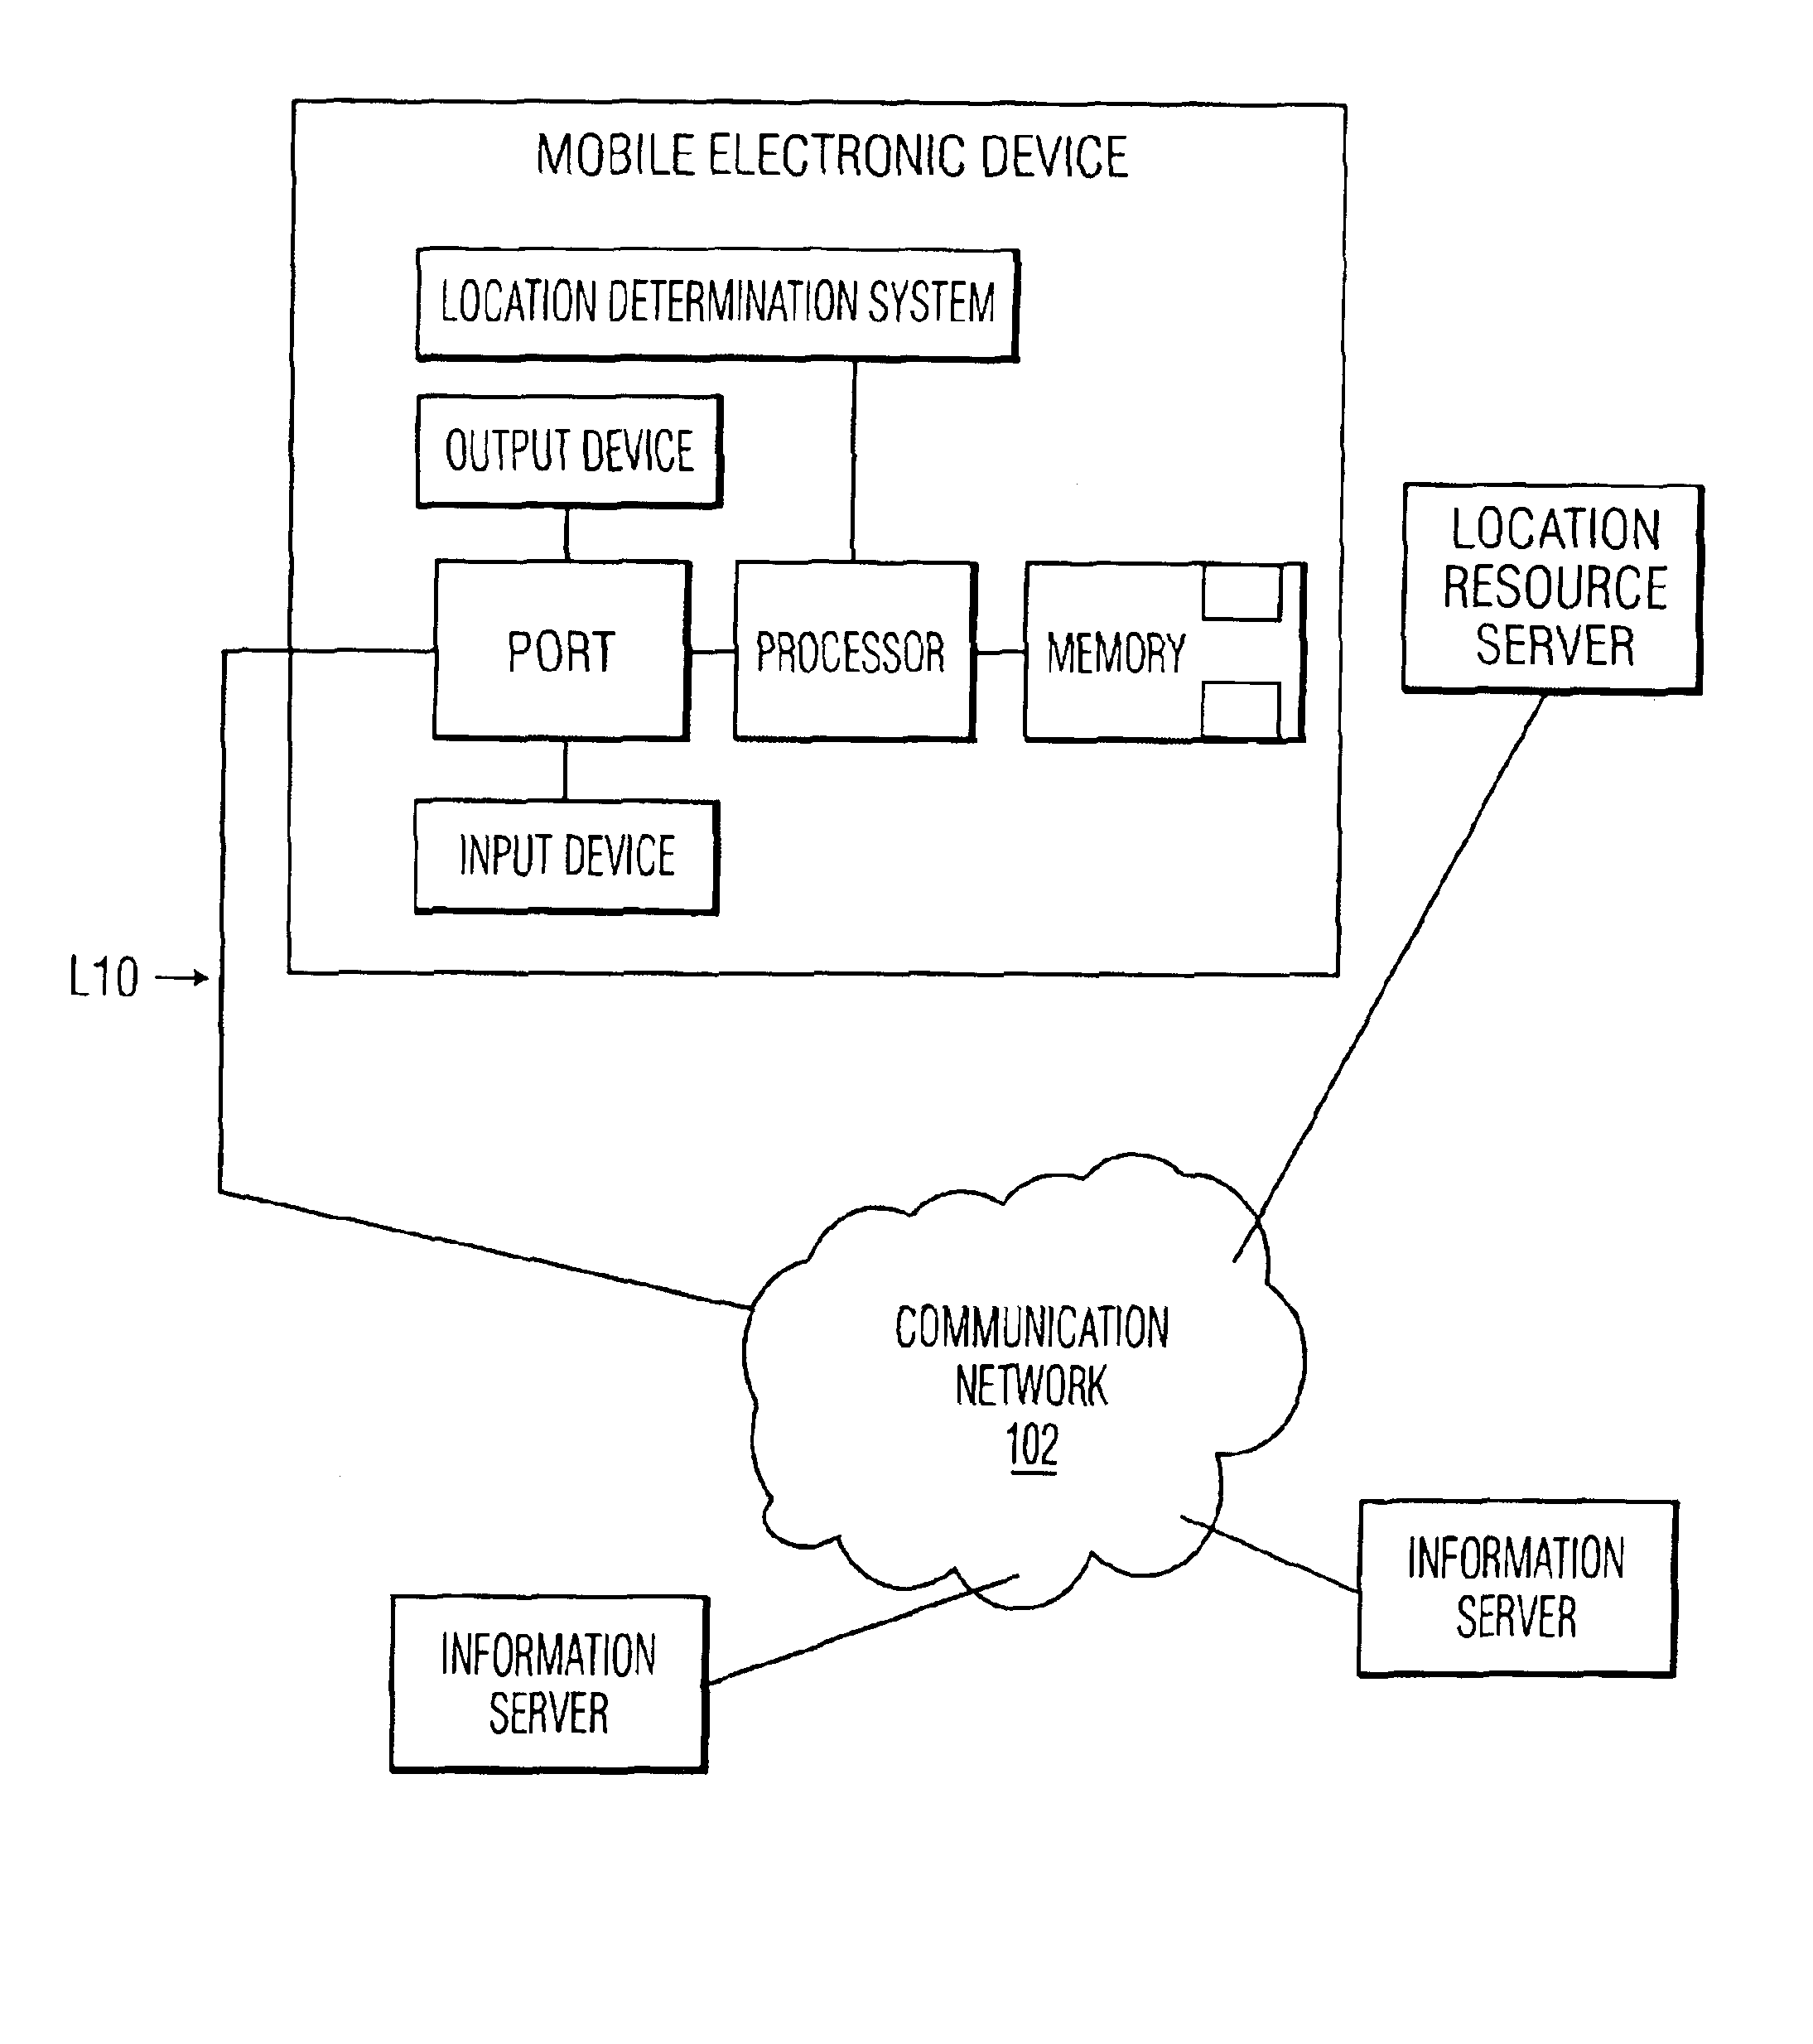
\includegraphics[width=300pt]{location}\\
    \caption{Diagram inquiring location \citep{rankin2005distributed}} \label{Figure: Diagram inquiring location}
\end{figure}

\par With this measure, the device can determine its current geographic location. A well-known method to provide the location determination function is to use a GPS receiver which is readily available in these phones, which can receive satellite signals to determine a location to within 10 meters of the user's location which has gotten better over the last number of years. GPS is the first kind of a self-contained location system. Another self-contained location system is a system which receives signals from nearby radio towers which are accurate to within 5km. The last is the internet connection to that device which can either be WiFi or mobile internet provided by the provider which is correct to within 50 meters.

\par The strategy provides the best kind of accuracy to battery life the ratio seems to be just correct compared to just using GPS which uses an astonishing 3.764Ws more than GPS by just using a WIFI network. During this project, we must use all three location strategies to enable the battery of the device to last the longest. By reviewing our previous research, this path seems. By examining our previous research, this route appears to be the correct path to take in comparison to using one strategy as this might inhibit our use of gaining the location of the device.\cite{bareth2011energy}

\section{Literature Conclusion}
Throughout this literature review process of gathering information from residual resources from different and also related fields. Such as the invention of the handheld modular phone, location strategies, cloud based services, and other Android applications that are on the same scale on which the developer is willing to produce incoherence with his Bsc(Hons) degree in computing. Due to the limited amount of time available for this project as follows, also with a small spectrum of fields that were discussed. It was somewhat difficult to find related projects on the same topic as the application itself. Which somewhat inhibited a wide-scale research on previous works associated with the project in question.

\par The concept of such project as a location-based historical, educational tool is rare as not many people would think of making applications like these, especially for a specific town. In recent years these applications are what clients need and want, also with new technology flowing through the markets smartphones are not a thing of the future they are readily available and don't cost that much to purchase.

\par Together with the methods of location strategies with respects to battery life and internet postage. The application is being developed at the correct time, As batteries would not last as long as they do now because of the cost of the processing power together with the integrated components of that mobile device. The code is now smarter in ways of allowing less idle time and microprocessors in these devices use a lot less power with more speed.

\par Of course, we can look at some of the many difficulties and concerns about mobile applications with the advances of malware with respects to privacy and reliability, but this field is growing and getting better with each day with the development of connecting everyone and their data together. Which is why when coding app's users have to accept what the app is trying to access specifically such as storage, location, wifi.

\par Together with the help of the IDE which contributes to helping the developer on coding the different classes of the app, and which also contributes to helping the developer in coding with the likes of the Google map API and firebase. Each needs a specific key to the API that is used which was expressed throughout the research of the project. 

\par The firebase cloud service helps the developer in managing user's and sending data throughout the system on updating the area's that are needed to display the information. With this in mind, databases can be easily updated and sent throughout the client base when that specific user logs in so that a larger update of the system is not needed on the google play store unless other graphical displays are in need of updating.

\chapter{Methodology Chapter}

\section{Appropriateness of the Research Design}
The following project was based on both a quantitative and qualitative approach to research techniques. Together with the amount of investigating completed collectively with this project before it had begun and throughout the developer received many high words of praise for an application of this type throughout the small and large suburbs of the Dublin area.

\section{Pilot Study of Proposed Project}
A pilot study of the application was first introduced to friends and family to get a sense of feel for if the application would be a good idea and to see if this is something that the people of Dublin would want to see coming to their mobile phones. Soon after getting a great response from family the developer chooses to produce a survey based on the people of Lucan. Based on the application and what if any specifications they would like to see. The developer received a response of over 150 people completing the survey on survey monkey. The application was indeed a certain choice for the developer to go ahead. Through wire-framing each screen that would be used throughout the application the developer had gotten an overall feel for what the end product should be.

\section{Ethical Considerations}
Each part of the project that has been carried through is deemed to be the developer's work unless stated otherwise. Other factors may contribute to the writing of this formal document and the project as a whole. Information that has to be gathered for the project as follows will be referenced appropriately. Such as that the monuments within the application itself will not be information that the developer has written but information that has been gathered from a third party. Such as an internet source which will be verified.

\section{Validity}
The data sourced for the project is to the developer's knowledge correct. Multiple sources have been read through and verified such data that is being used. Articles such as journals and other particles of information were referenced throughout to the original authors that the information was taken from or sourced.
\section{InforMe@Dublin Survey Results}
Regarding the following chapter which discussed the methodologies of why the developer chose to develop an Android application for the intended use on patrons learning about historical monuments in their area's. The results are as follows. The following survey was completed using survey monkey.

\begin{figure}[!tbp]
    \centering
    \begin{minipage}[b]{0.4\textwidth}
        \includegraphics[width=250pt]{Survey1}\\
        \caption{History Survey} 
        \label{Figure: History Survey}
    \end{minipage}
    \hfill
    \begin{minipage}[b]{0.4\textwidth}
        \includegraphics[width=250pt]{Survey2}\\
        \caption{History Survey} 
        \label{Figure: History Survey}
    \end{minipage}
\end{figure}

\begin{figure}[!tbp]
    \centering
    \begin{minipage}[b]{0.4\textwidth}
        \includegraphics[width=250pt]{Survey3}\\
        \caption{History Survey} 
        \label{Figure: History Survey}
    \end{minipage}
    \hfill
    \begin{minipage}[b]{0.4\textwidth}
            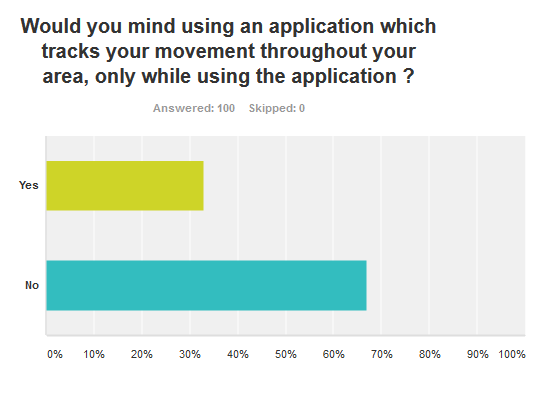
\includegraphics[width=250pt]{Survey4}\\
            \caption{History Survey} 
            \label{Figure: History Survey}
    \end{minipage}
\end{figure}
\newpage
\section{Summary}
The following chapter of which, concluded the research that has gone into choosing such a project in coherence with the BSc(Honours) Degree programme in the Institute of Technology Blanchardstown. The following was to see if the application that the developer had invented was deemed appropriate and needed in the area of Dublin. With the facts stated and nothing of the sort available online from other countries or in fact Ireland. The projects seemed plausible if the developer could, in fact, produce something of the application in mind.



\chapter{System Requirements and Specification}

\section{Description}
Throughout the following chapter, the system designs of the project will be represented as diagrams. Using use-case diagrams, Activity diagrams and sequence diagrams with descriptions of these such diagrams displayed throughout the chapter as an aid in understanding the communications between each specific component of the app. These are needed for the reader to be able to comprehend the app as a whole. 

\section{Underlying Architecture of the Android OS}
Regarding the underlying architecture on which an application will be in fact lying on top of the Android operating system. The following operating system is, in fact, a stack of software components which are mapped in coordinance with the corresponding hardware modules at the Linux kernel layer. The software stack is roughly divided into five specific sections and four different layers of which the frameworks, libraries, kernel and applications sit. The following diagram in figure 5.1 shows this. 

\begin{figure}[htbp]
    \center 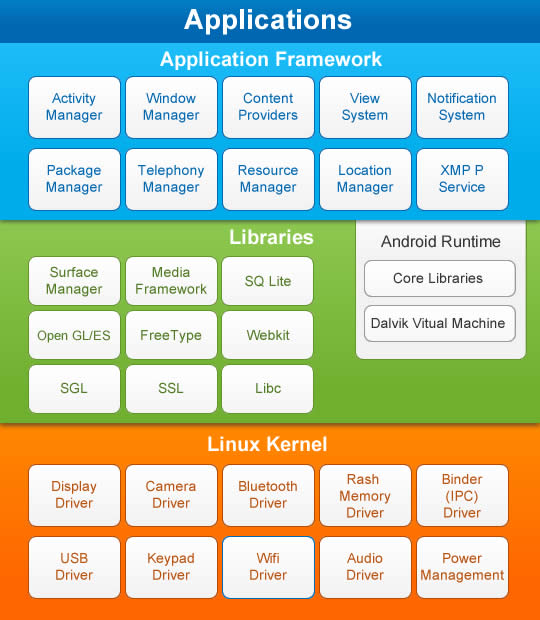
\includegraphics[width=400pt]{AndroidOS}\\
    \caption{Android Architecture \citep{androidlife}} \label{Figure: Android Architecture}
\end{figure}
\par 
Concerning the Linux layer of the following OS. The version of which is Linux 3.6 on which has approximately 115 patches to its name. This layer acts as a level of abstraction between the devices software modules and its hardware components on which contains the following, camera module, keypad, display, GPS and a wifi module, etc. Utilising the fact that Linux is a great source for networking and on which supports a vast array of drives which provided a solid base on providing a somewhat reliable OS.

\section{Android's Incorporated libraries}
Concerning the libraries of which are incorporated within the application these apps are used to retrieve information on which may be related to specific applications on the device. On top of the Linux kernel, there are a set of libraries which includes an open source web engine WebKit, libc which is a standard C library which was created by Google for its Android OS and also an SQLite database of which is a useful repository for storage and sharing of application data throughout the program. Other libraries also include SSL which is responsible for the security of the device with regards to internet connectivity. Other libraries are also included to record and play audio and video.
\section{A Look at Android's Location Service's}
Utilising a client's mobile device on gaining their exact location can be done in two ways one of which is favoured over the other. The first way of allocating the user's location can be done by utilising the GPS module of the device by using Android's built-in Location API's which have been available since Android's first launch. These location gathering API's still work even to this day. However, uses a lot of the device's power to gain specific coordinates. With the following in mind, the user must more likely be outdoor's for the following to work to get a signal to a GPS satellite.

\paragraph{Google Play Services} -
The developer of the application InforMe@Dublin has utilised a new way of gaining clients geographical coordinates by way of using Google Play Services of which provides a very powerful, high-level framework to work from. This provides a choice of location gathering tools, such as WIFI and internet connection, GPS modules, cellular fixation or to bundle these together to provide a more accurate location fixture. The following API allocates power management of the device to keep each mobile phone at the top of its game.
\par
Android gives applications of which access location services supported by the device through classes in the android.location package. The most important component of the following framework is the LocationManager which is a system service related to figure 5.1. The following provides APIs for determining the location of which the device is in at that current time. The digram located in figure 5.2 shows how the location service and manager work together with the system in order to retrieve the devices location.

\begin{figure}[htbp]
	\center 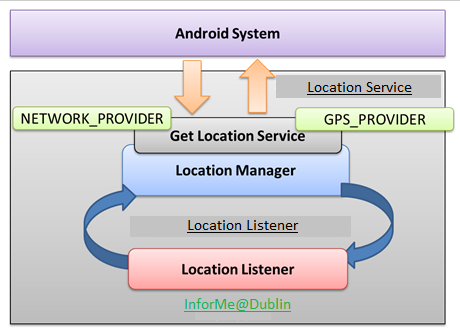
\includegraphics[width=400pt]{locationManager}\\
	\caption{Retrieving Location} \label{Figure: Retrieving Location}
\end{figure}


\section{Installation of InforMe@Dublin}
Before the user accessing the following application, the app may first be downloaded from the Google play store on which the developer has chosen to release to the general public. The application would be available or work for people living in the Dublin area. When the application has been downloaded and of the installation being completed the following diagrams will show how the system works.

\section{Login and Authentication Diagrams}
The following diagrams represent the application's login page as well as some various activities on which the user may enter before moving forward while using the application.

\subsection{Login Use Case Diagram}
Regarding the Use Case diagram in figure - 5.3, The reader can grasp the associated activities that are compiled within the login page. When first starting the InforMe@Dublin application the user may only use the following activities to gain access to the map area of that app. Which are Google sign in, Creation of an account, forgotten password of an existing account or to log in with the user's credentials if account already created.\par

\begin{figure}[htbp]
    \center 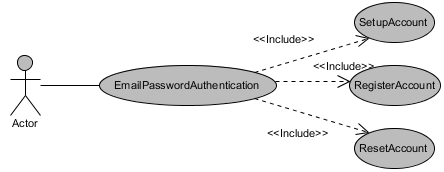
\includegraphics[width=450pt]{EmailAndPasswordUsecase}\\
    \caption{Login Use case Diagram} \label{Figure: Login Use case Diagram}
\end{figure}

\subsection{Login Activity Diagram}
Regarding the following Activity Diagram in figure - 5.4, The developer has produced an activity diagram displaying how each component works with one another. As the following classes and activities are seen is how the source code is laid out. Each specific part of the Android app has its specific package for the purpose of modularity. While visualising the diagram the reader can distinguish how each of the specific button clicks are mapped. Each specific activity has its very own methods on which the user must specifically progress through to gain access to the signed in activities these specific buttons and menus are hidden until the client has been authenticated by firebase's authentication method which is located in the EmailPasswordAuthentication activity.
\begin{figure}[htbp]
    \center 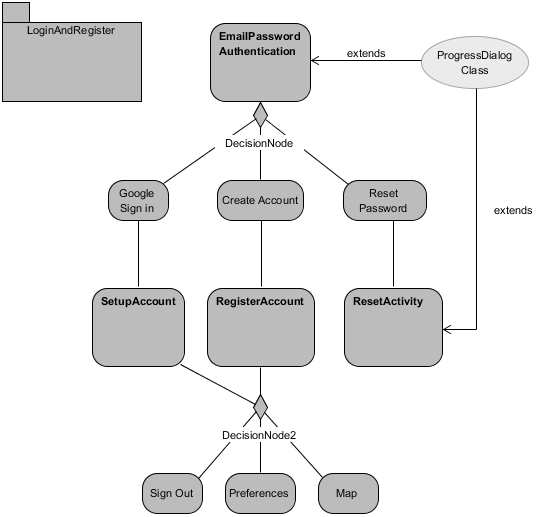
\includegraphics[width=450pt]{Login&RegisterActivity}\\
    \caption{Login Activity Diagram } \label{Figure: Login Activity Diagram}
\end{figure}

\subsection{Login Sequence Diagram}
Regarding the sequence diagram located in figure 5.5, The Reader can comprehend what tasks are being processed in the background by their actions on which they are pursuing. While starting the application and looking at the following diagram the reader can see the generic association between the actor and the EmailAndPasswordAuthentication activity which is created on starting the app. Which checks immediately if a user was already signed in using the mobile device and have not specifically signed out which allows the user to access a new set of activities which enable them to discover Dublin in a new light and to find hidden monuments that have stood the test of time.\par

\begin{figure}[htbp]
    \center 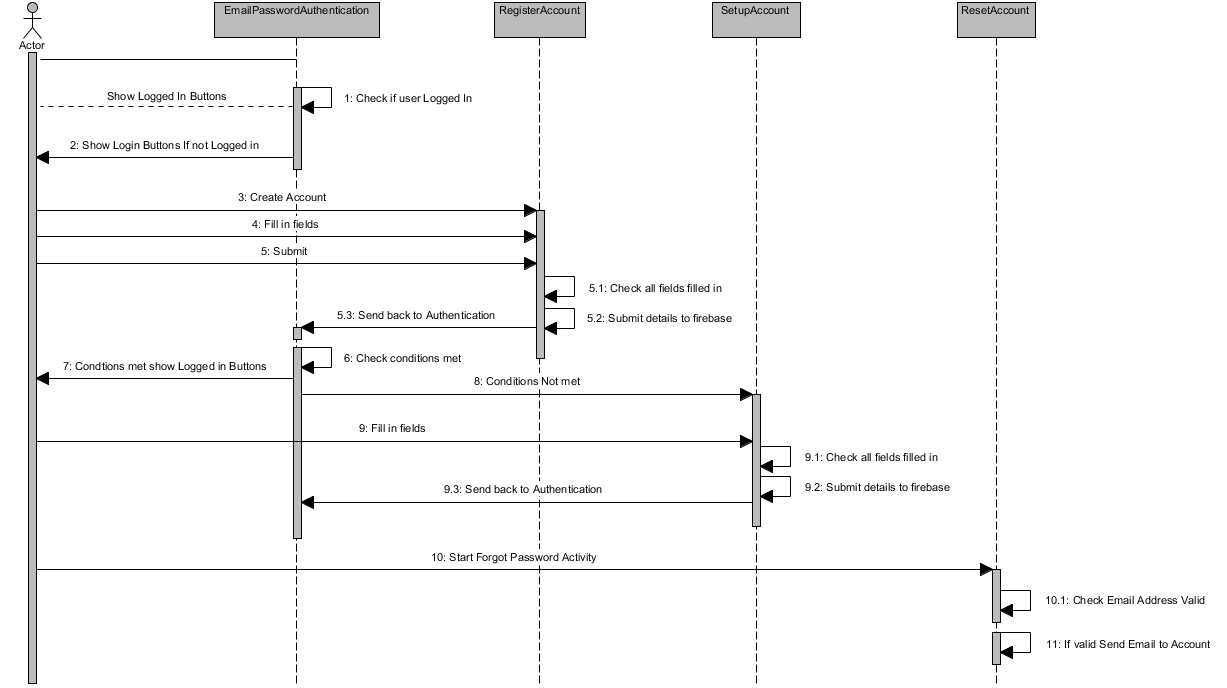
\includegraphics[width=500pt]{Login&RegisterSequence}\\
    \caption{Login Sequence Diagram } \label{Figure: Sequence Diagram}
\end{figure}

\par
While looking at the different activities on which the user may take there are also associated checks which need to be performed to proceed to the next area of the application. Even when a new user creates an account the following account needs to be verified with the Firebase database to check if such a user exists this is not just for authentication but to enable users to post their accurate information with an allocated name, profile picture and unique ID which distinguish's them from other users. When a user has either created an account by registering with an indifferent email address or signing in with the aid of Google sign in, on the authorization of the account The user is brought back to the EmailAndPasswordAuthentication Activity. On which the user is validated, and new options are then shown to the user for them to proceed to the MapActivity or to change preferences as well as signing out of the application.

\section{Maps and Geofencing Diagrams}
The following section is to show using diagrams how the maps and geofencing activity works and its associated classes and activities that are combined to retrieve notifications on which a user has entered a specific geofence. With hence to its specific class, the maps activity must have an allocated map fragment which is defined on the designed layout that is accessed by a reference by the class to produce a suitable map. On gaining the Location of the device we first need to check the permissions of the application especially if the device is using Android Marshmallow or above. As there are new permission intents on which the user must explicitly accept to use specific components of such device. When these permissions have been accepted the application then has access to the GPS module located in the device which most mobiles have in this day and age. With these specific settings turned on and with the permissions set in hand, the app is then available to accept location updates which are set on that activities class and are updated by specific intervals which are set by the developer. These are just a few of the methods that the developer will run through on the next chapter but for now the diagrams of communication between the user and device.

\subsection{Maps and Geofence Use Case Diagram}
While viewing the following use case diagram located in figure 5.6, the reader can see that it is quite an easy diagram to comprehend as there are only three use cases that can be seen on which the user can use with specific button clicks. The main area of this map activity is to utilise the GPS locator of the device to receive updates on whether the user has entered a geofence location which a notification and dialogue pop-up will appear to the user entering such an area.

\begin{figure}[htbp]
    \center 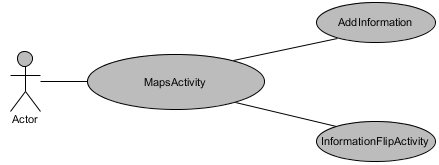
\includegraphics[width=450pt]{MapsUsecase}\\
    \caption{Maps \& Geofence Use Case Diagram } \label{Figure: Maps & Geofence Use Case Diagram}
\end{figure}

\subsection{Maps and Geofence Activity Diagram}
We can see by looking at the following diagram figure 5.7, on which how each specific component is mapped to the main MapsActivity which does all of the computation with regards to retrieving a location from the device which allows for this app to be a location aware application. While looking at the two reference classes and distinguishing what if anything they do is simple. The Place class utilises the notification thrown when a user is in a geofence. The maps activity acts as a broadcast receiver to retrieve the information which a pending notification intent was thrown populates the Place methods with the name of the area which a notification was thrown and passed to the InformationFrontActivity when the users choose to enter the specific monuments activity.\par

\begin{figure}[htbp]
    \center 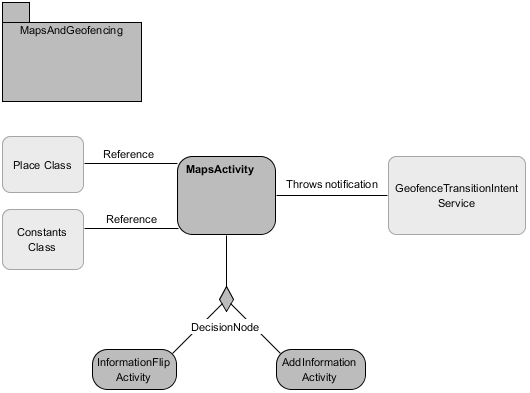
\includegraphics[width=450pt]{MapsGeofenceActivity}\\
    \caption{Maps \& Geofence Activity Diagram} \label{Figure: Maps & Geofence Activity Diagram }
\end{figure}
\newpage
\subsection{Maps and Geofence Sequence Diagram}
The following sequence diagram located in figure 5.8 represents the states of which the user will be initiated through with hence to the background workings of the application. While viewing the diagram, the reader can see the initial connection between the user and MapsActivity.  Which the onCreate of that specific activity triggers methods which set up the map fragment, adding geofences which are retrieved from firebase, GoogleApi which is needed to request the location from the user's devices as well as the connectors to the camera view to adjust the camera view of the map on location changes. With this in mind when the location changes the application renders whether the application has entered a geofence location. On going into a geofence, a pending intent will be initiated which will then trigger a notification which will display on the user's device. The user may want to view the information or not it is not compulsory to view the information on the application. Another opportunity on which a user might want to undertake is to send information to the InforMe@Dublin Gmail account to add more geofences with images and information to the InforMe@Dublin Android Application.\newpage

\begin{figure}[htbp]
    \center 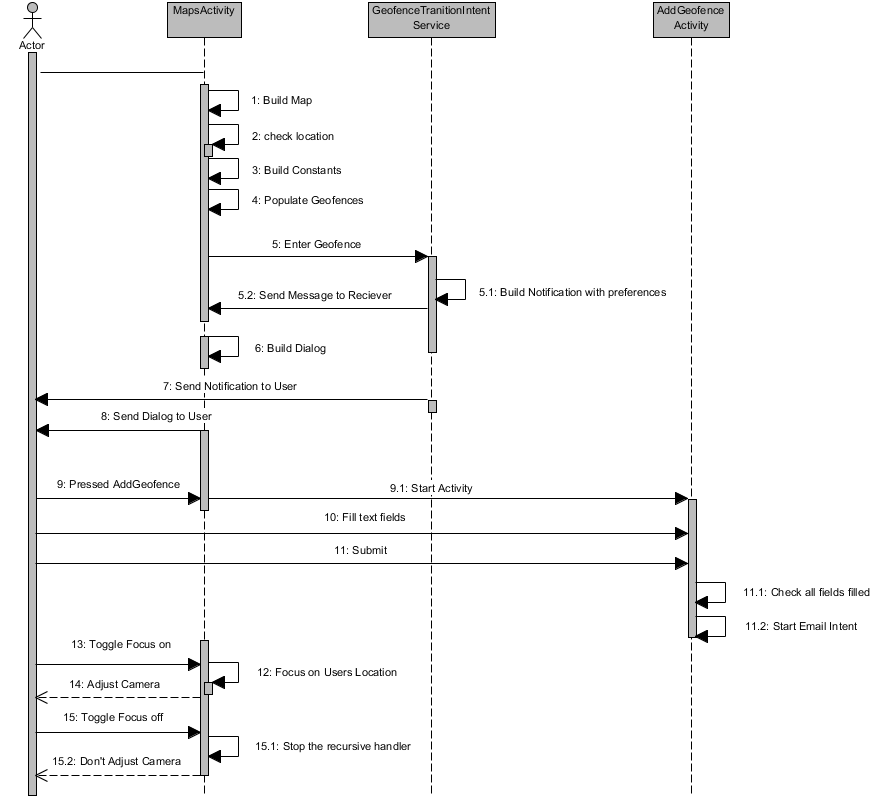
\includegraphics[width=400pt]{MapsSequence}\\
    \caption{Maps \& Geofence Sequence Diagram} \label{Figure: Maps & Geofence Sequence Diagram }
\end{figure}

\section{Information and Posting Diagrams}
During the following phase of the project is where the user can view the information of the monument on which they have entered and post some information about that specific area if they wish while they are in the same vicinity of the monument. These fragments which are created when the user selects to view the information on the specific area. On using the icons which change the view of each fragment activity when on the informationBackCommentsFragment is on the main view users can then choose to Post comments, update comments or just to view the post as a whole without other posts in the way. The following Diagrams will display how each component works together to retrieve information for where exactly the user is located.

\subsection{Information and Posting Use Case Diagram}
Regarding the following diagram figure 5.9 showing the use case diagram as shown distinguishes how each of the user's actions is mapped on clicking certain buttons which were applied to the layout file and linked to the activity. On entering the InformationFlipActivity, the user is sent to the InformationFrontFragment which displays the information of the monument of which the user has entered the specific geofence. The user can only access these specific activities on entering from an allocated geofence.\par

\begin{figure}[htbp]
    \center 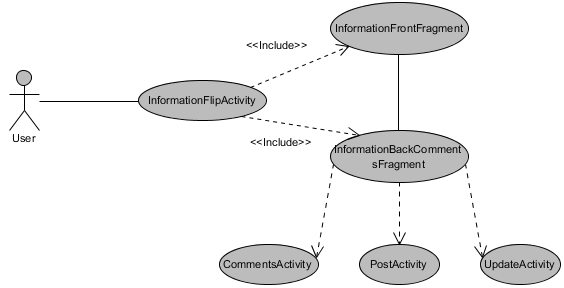
\includegraphics[width=350pt]{PostingAndInformationUsecase}\\
    \caption{Information \& Posting Use Case Diagram} \label{Figure: Information & Posting Use Case Diagram }
\end{figure}

\newpage

\subsection{Information and Posting Activity Diagram}
Regarding the Activity diagram in figure 5.10, the reader can see how each part of the package PostingInformationAndComments the classes as follows in the diagram. The InformationFlipActivity controls both InformationFrontFragment and InformationBackCommentsFragment both of these fragments are controlled using the menu bar of these fragments the InformationFlipActivity uses a stack to flip each of the fragments back to front. Only when the InformationBackCommentsFragment is displayed may the users create and view posts made by other users and also themselves When viewing the posts, the user can then like specific posts that have been created by the user or other users.\par

\begin{figure}[htbp]
    \center 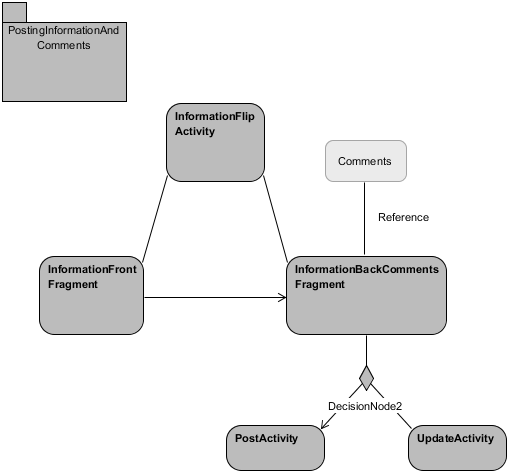
\includegraphics[width=350pt]{PostingInformation}\\
    \caption{Information \& Posting Activity Diagram} \label{Figure: Information & Posting Activity Diagram }
\end{figure}

\newpage

\subsection{Information and Posting Sequence Diagram}
Looking at the diagram in figure 5.11 the reader will grasp a better understanding of the following Activities on viewing the information of the specific monument as well as viewing the posts which are retrieved using firebase methods on which the developer will discuss in the following chapters. On entering the front fragment, the following methods are then initiated on starting the activity such as retrieving the information from the Firebase database which has been referenced to the specific JSON file. The fields of the activity will then be populated with the information which has been retrieved as well as images being loaded with specific URL's which have been saved in a hashmap and loaded within a page scroller. On viewing the posts from the user, these are populated by using the InformationBackCommentsFragment as well as the Comments class to populate the data and to display in a page view of specific user's posts which were posted on that monuments page.\par

\begin{figure}[htbp]
    \center 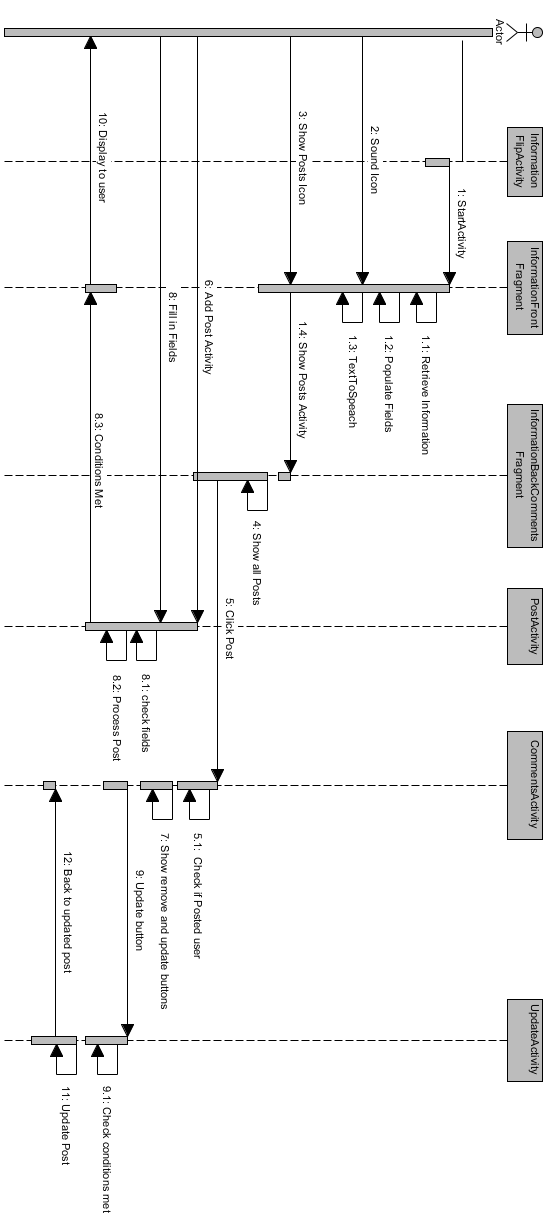
\includegraphics[width=250pt]{PostingAndInformationSequence}\\
    \caption{Information \& Posting Sequence Diagram} \label{Figure: Information & Posting Sequence Diagram }
\end{figure}

\newpage

\section{Settings Diagrams}
The following diagrams regarding the settings preferences are discussed throughout this section of the chapter. With hence to the settings activity, the user can change the application's preference with regards to setting the vibration of the notification which is sent on entering the geofence. The user can also change the notification sound as well as a battery save mode which utilises the proximity sensor to sense if the device's screen is on and if the sensor of the device is covered.

\subsection{Settings Use Case Diagram}
The following diagram shows the reader how the Settings and activities that are combined within the preference activities which allow the user to change specific settings for that application the user can change the settings as follows with the following activities as shown in the figure 5.12.\par

\begin{figure}[htbp]
    \center 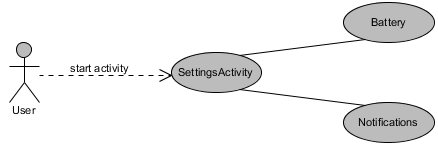
\includegraphics[width=450pt]{SettingsUsecase}\\
    \caption{Settings Use Case Diagram} \label{Figure: Settings Use Case Diagram }
\end{figure}

\subsection{Settings Activity Diagram}
The following diagram located in figure 5.13 shows the reader how the Settings and AppCompatActivity reference to each other when changing the preferences of the user. The CheckConnectivity class represents the application to see if the device is connected to the internet and if the Gps module is activated.

\begin{figure}[htbp]
    \center 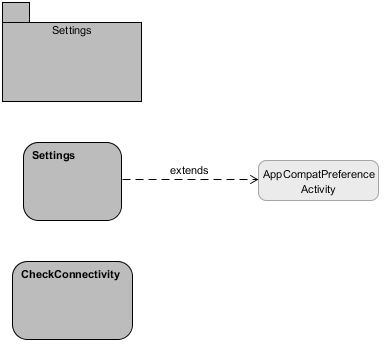
\includegraphics[width=350pt]{SettingsActivity}\\
    \caption{Settings Activity Diagram} \label{Figure: Settings Activity Diagram }
\end{figure}

\subsection{Settings Sequence Diagram}
While viewing the following diagram located in figure 5.14 shows how the user associates with the settings Activity while utilising the preference layouts as well as the AppCompatActivity this then shows the preference which will be discussed in the next chapter of this thesis. 

\begin{figure}[htbp]
    \center 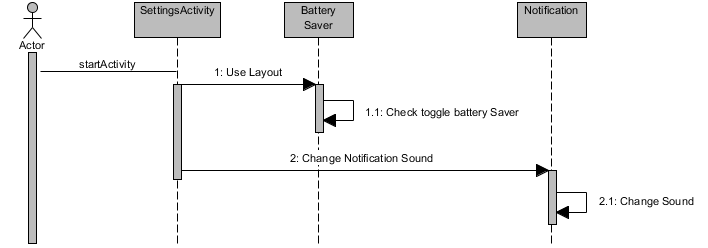
\includegraphics[width=450pt]{SequenceDiagramSettings}\\
    \caption{Settings Sequence Diagram} \label{Figure: Settings Sequence Diagram }
\end{figure}

\section{Overall System Use Case Diagram}
The following diagram represents the InforMe@Dublin application as a whole. Concerning the following use case diagram located in figure 5.15, the reader can then see all of the different components on which a user can enter within the constraints of being signed in and with the submission of posts by the specific user being able to remove and update their specific posts. The reader can see how each component is connected to each other and on where the user can gain access to certain activities throughout the following application.\par

\begin{figure}[htbp]
    \center 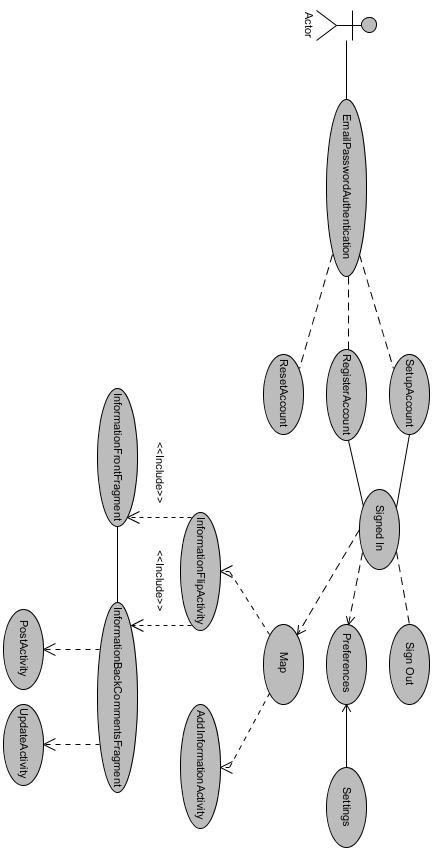
\includegraphics[width=300pt]{FullActivityUseCase}\\
    \caption{Overall Use Case Diagram} \label{Figure: Overall Use Case Diagram }
\end{figure}

\newpage

\section{Activity Diagram with Overall System}
Regarding the diagram figure 5.16, The activity diagram as a whole is to show the reader how each component is used throughout the system to grasp a better understanding of which Activities and classes are working and what exactly is each of these specific items doing throughout the Android application. When brought together as a whole with descriptions of each package and the associated classes and activities the reader may gain a better understanding of the following project. The InforMe@Dublin Android application is not meant to be complex in nature but descriptive enough to show the findings the developer designed within the application.

\begin{figure}[htbp]
    \center 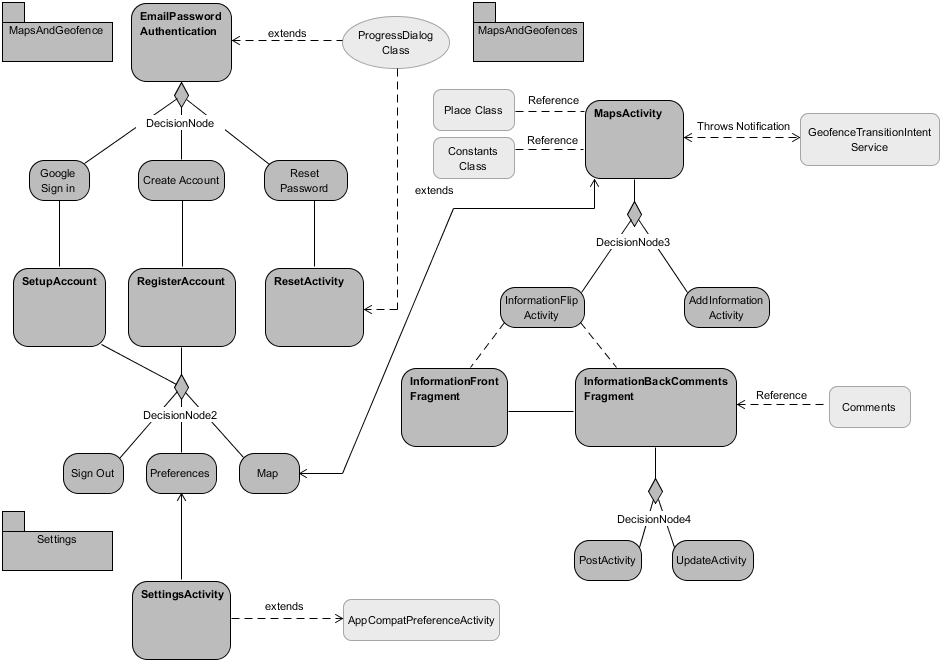
\includegraphics[width=470pt]{FullActivity}\\
    \caption{Overall Use Case Diagram} \label{Figure: Overall Activity Diagram }
\end{figure}


\section{Summary of the Chapter}
Throughout the following chapter, the developer has brought us through the different steps of how the user can interact with the application as a whole, and of which components of the app are connected to one another. Another aspect that the developer has to show us is the communication between the application within the packages of which are of a modular concern to the specific components of the app, concerning the MapsAndGeofence package holds all the classes and activities which are only used once a patron of the application is in that specific activity. With that in mind, the developer hopes that the reader understands how the application is mapped out and thoroughly understands of which the developer is trying to achieve. The next chapter of the following thesis is to show the wireframing and design aspects of the InforMe@Dublin Android application with hence to colour schemes and layouts of each specific activity.

\chapter{Application Design}

\section{Description of the Chapter}
The following chapter discusses the design of the application, with regards to layout and colours used throughout each page. Within the chapter, the developer will provide wireframes with regards to the thought process of the layout resource files. The Logo of the application will also be discussed with the reason behind the naming of the application provided below.

\section{Creation of InforMe@Dublin's Logo}
The inspiration for the InforMe@Dublin came from the using Google maps location markers of which is an iconic symbol to use of which ties into the following application quite well as it utilises maps and a mobile devices real-time location. The naming of the application is as the name state's to inform someone about something which in this case is the county of Dublin. The colours of which are used in the logo were just clean and crisp looking of which complimented the other parts of the logo. Other colours that were tried just didn't tie in with the look and feel of the application.

\begin{figure}[htbp]
	\center 
\includegraphics[width=150pt]{informe}\\
	\caption{InforMe@Dublin Logo} \label{Figure: InforMe@Dublin Logo}
\end{figure}
\newpage
\section{Start Page}
While designing the startup page of the application, certain permissions are requested in order to retrieve the device's location for the application being able to use the GPS module and to access the storage of the Android phone. The following wireframe represents the application after the installation has been completed and opened the following screen will be shown to the user. While looking at the following wireframe located in figure 6.2, The logo is the first aspect of the application on which the user should see which represents what the app is actually about the layout is also smooth and well round

\par 
Looking at the wireframe which was designed by the developer the reader can see where the user may log in with their credentials as well as using OAuth sign in by linking their personal Gmail account which continues to the setup of an individual account on the InforMe@Dublin app. The button is in the lower centre of the page with the button Google sign in. With regards to the login activity, the layout is a relatively appealing design.

\begin{figure}[htbp]
    \center 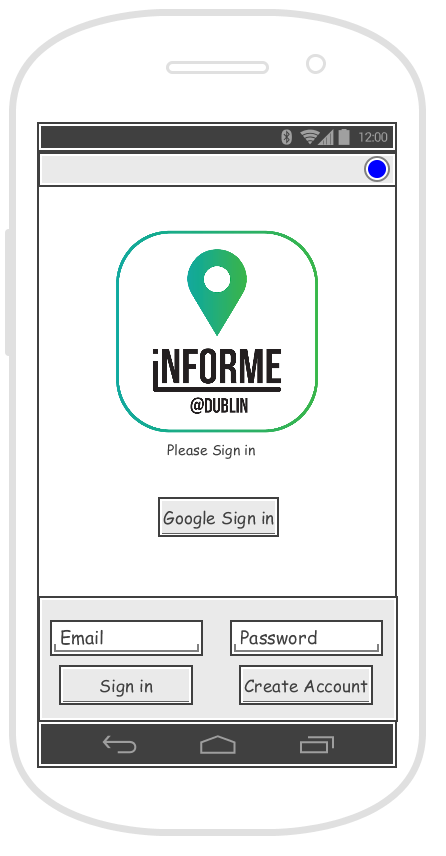
\includegraphics[width=150pt]{LoginWireframe}\\
    \caption{Login Wireframe} \label{Figure: Login Wireframe}
\end{figure}
\newpage
\section{Colour Scheme}
After looking at the first screen login wireframe. The developer would like to display the colours of which will be used throughout the app the colours are as follows. The developer chooses these specific colours as it complements the project as a whole. Are used throughout the multiple pages with are incorporated throughout the app. The following colours make for a sleek look while users are utilising the app.

\begin{enumerate}
    \item Theme of Application - R 43 / G 152 / B 212
    \item Buttons of Application - R 249 / G 159 / B 27
    \item Logo of Application - Blue: = R 0 / G 167 / B 157    Green: = 56 / G 180 / B 73 
\end{enumerate}    

\begin{figure}[htbp]
    \center 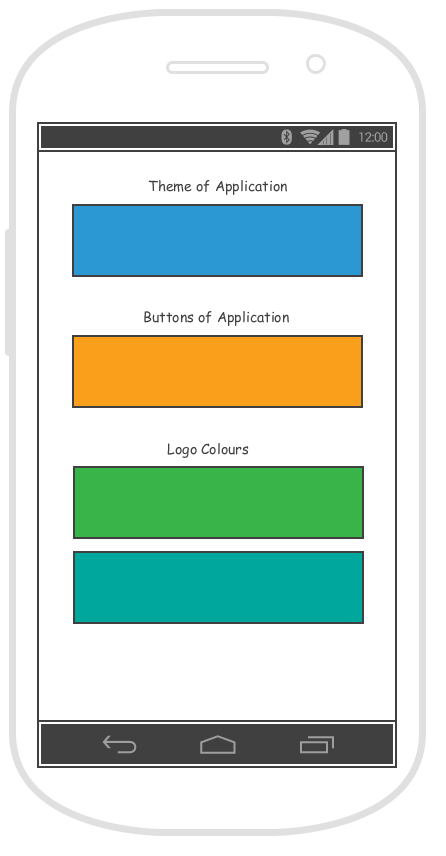
\includegraphics[width=150pt]{ColoursWireframe}\\
    \caption{Colours Wireframe} \label{Figure: Colours Wireframe}
\end{figure}

\section{Wire-frames}
The wireframes in this section of the chapter are regarding the wireframes on which were created by the developer. These wireframes were meant as a guide on how the layouts of the different activities would look like on completion of the application in question. Each styling aspect of the application was followed throughout the development. All colours used were disclosed in the above section.

\subsection{Login}
The following logged in wireframe is to be used in conjunction with the login wireframe which will authenticate the user as well as sign in the user of the application. Different display buttons will be shown to the user on authentication with both firebases authentication and the database of the Firebase API.

\begin{figure}[htbp]
    \center 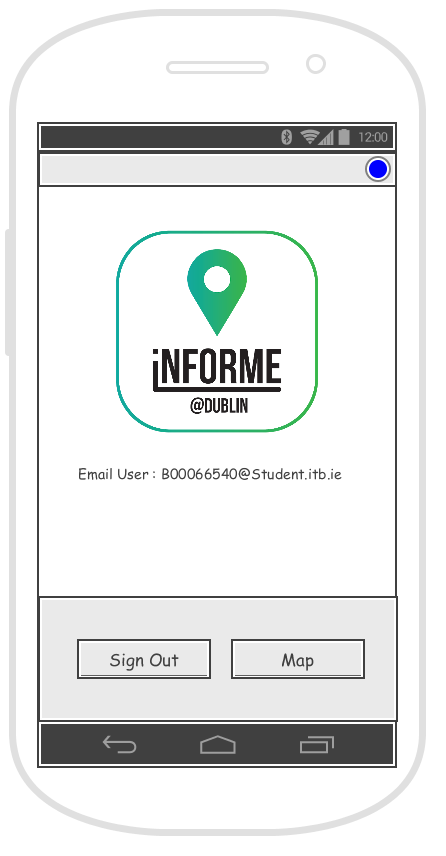
\includegraphics[width=150pt]{LoggedInWireframe}\\
    \caption{Logged in user Wireframe} \label{Figure: Logged in user Wireframe}
\end{figure}

\newpage

\subsection{Map}
With regards to the Maps Activity wireframe on which was designed by the developer, shows were the specific buttons are for the user throughout the using of the application. While viewing the wireframe, the reader can then distinguish how the real activity will be laid out. On the left-hand corner of the activity shows the compass area on which the user can choose to use. On the right-hand corner is used to toggle the focus of the user's location on which changes the camera animation to the devices current location utilising latitude and longitude. With regards to the bottom half of the screen on the bottom left-hand side of the display is where users can choose to send information to the InforMe@Dublin developer to update the Firebase database to add more historic locations for other users to enjoy.

\begin{figure}[htbp]
    \center 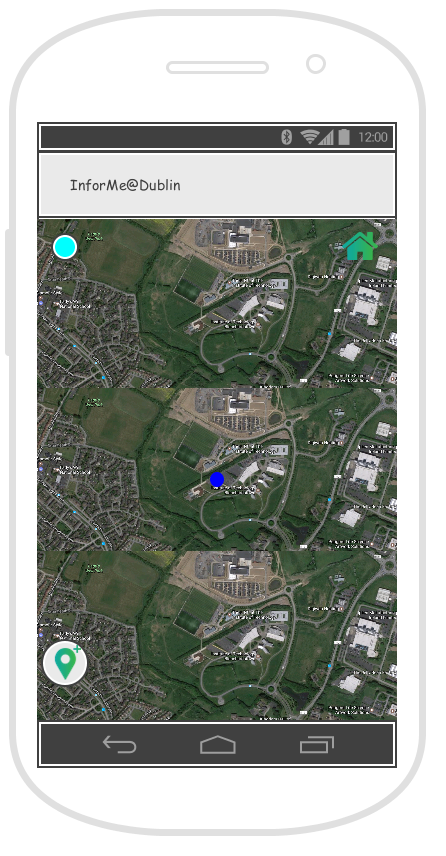
\includegraphics[width=150pt]{MapActivityWireframe}\\
    \caption{Map Activity Wireframe} \label{Figure: Map Activity Wireframe}
\end{figure}

\par
The next wireframe in this section shows what happens when the user has entered a particular geofence a dialogue is displayed with the monuments name on which the user of the application can then continue to view the information on the specific location on which the dialogue appeared for. A notification will also be sent on entering the location which is a general notification of the application notifying the user of a geofence on which they have entered.

\begin{figure}[htbp]
    \center 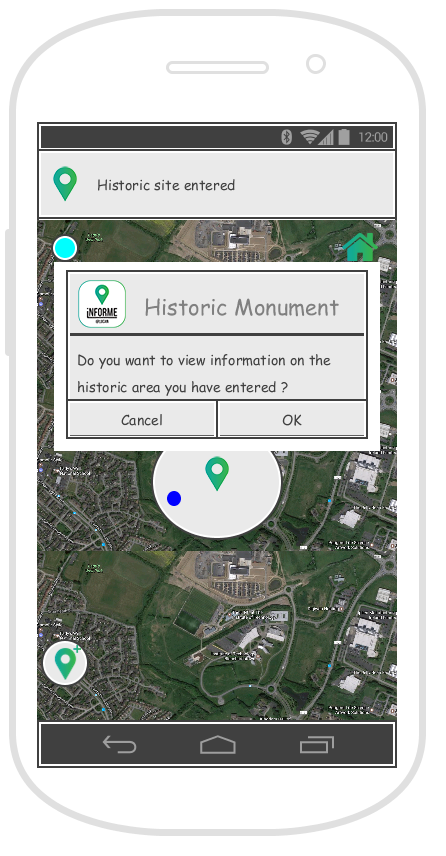
\includegraphics[width=150pt]{GeofenceMapWireframe}\\
    \caption{Map Activity Geofence Wireframe} \label{Figure: Map Activity Geofence Wireframe}
\end{figure}

\newpage
 
\subsection{Settings}
The following section of this chapter represents the settings page of the application with a more particular reference to the preferences of the application. Within the following wireframe, the following preferences can be changed in the activity that is related to the application.

\begin{figure}[htbp]
    \center 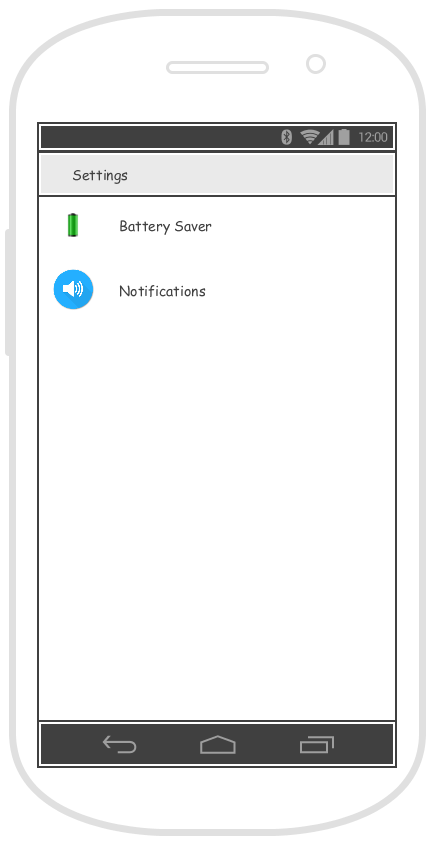
\includegraphics[width=150pt]{SettingsPreference}\\
    \caption{Settings Preferences Wireframe} \label{Figure: Settings Preferences Wireframe}
\end{figure}

\subsection{Add Information}
Concerning the following figure 6.8 shows the design on which will be implemented on the InforMe@Dublin app. with the wireframe in mind the user will be able to fill in the fields that are necessary for the app to create an email and send to the developer of the application. By pressing the select images button, the users will be brought to their personal gallery on which they can choose images to post to the developer as well as any information they might have at hand such as the location of such monuments.

\begin{figure}[htbp]
    \center 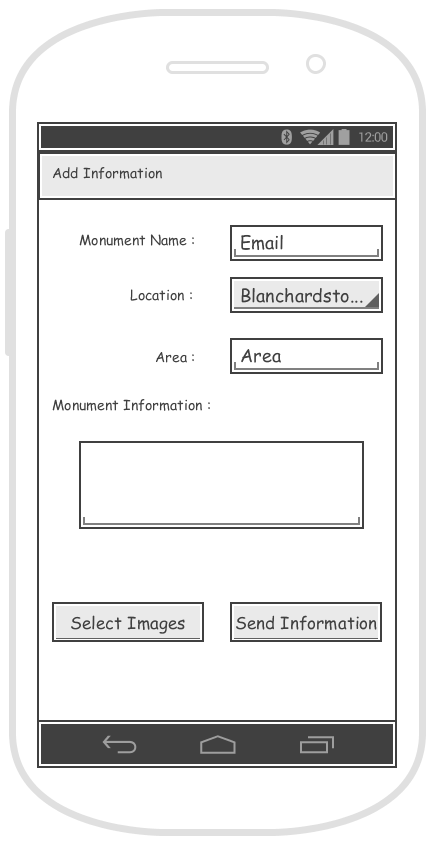
\includegraphics[width=150pt]{addInformationWireframe}\\
    \caption{Add Information Wireframe} \label{Figure: Add Information Wireframe}
\end{figure}


\subsection{Show Information}
With relation to the following section located in the system design. Two wireframes were developed in which the developer of the application could get a better understanding of what he wanted to achieve. The following wireframes were turned into resource layout files to complete the look and feel, and the developer thought that these following layout files would be the most important design in such an application. Information is the most important factor in the project which needs to be portrayed to the user in a specific manner. Creating a crisp clean and non-cluttered layout was the key ingredient which why the wireframes layout below was chosen.
\par
While looking at both figures 6.9 and 6.10, the reader can see the distinctive feel of what the developer is trying to achieve by using both of the following activity wireframes as fragments the developer can create a smooth turn around feel of the information on which the users want to see. While looking at figure 6.9, users can get to grasp with the images that have been used from multiple sources. The information that the reader can see is just filler text that was generated from a website. Were the filler text is in the wireframe is compiled of the information from that monument which was sourced from multiple sources on the internet. A button which is shown as a loudspeaker icon will then perform a text-to-speech on the information which was retrieved from the Firebase database.

\begin{figure}[!tbp]
    \centering
    \begin{minipage}[b]{0.4\textwidth}
        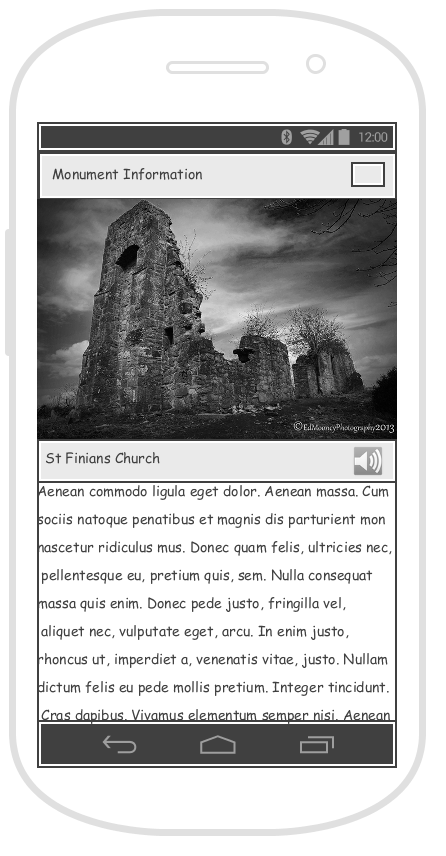
\includegraphics[width=\textwidth]{DisplayInformationWireframe}
        \caption{Display Information }
        \label{Figure: Display Information }
    \end{minipage}
    \hfill
    \begin{minipage}[b]{0.4\textwidth}
        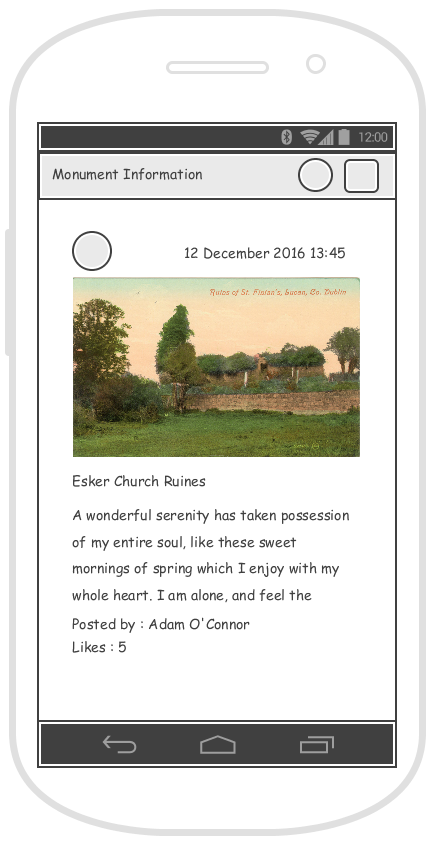
\includegraphics[width=\textwidth]{ViewPostsWireframe}
        \caption{View Posts } 
        \label{Figure: View Posts }
    \end{minipage}
\end{figure}

\section{Summary of the Chapter}
To conclude the chapter as a whole, the reader can see that the developer has discussed the design of the InforMe@Dublin application. Each page of the app has been mocked up which allowed the developer to visualise how it should look at the end of development. While providing these wireframes in this current chapter, the reader can grasp a much better understanding of how the application prototype will evolve throughout the time of development and also with regards to the time scale allowed on which the final build and release of the project will be of the date 27th of April. The next chapter in this thesis discusses the coding of the application on the loading of geofences, providing permissions to the user on Android Marshmallow OS and above and many more feature on which were incorporated into the app. Each separate part of the next chapter will be discussed with regards to the different methods of which are associated with its specific method. 
\chapter{Implementation of System}

\section{Initialization of the System}
The installation of the application is available on the google play store, the name of the application is InforMe@Dublin and is created under the company Smooth Solutions which is the name of which was created by the developer Adam O'Connor.

\section{Background to Android Devices Activity's Life-cycle} 

Regarding the activities on which each of these specific sections in the following chapter is based on a single activity page where all these methods are then utilised. The Android Activity Lifecycle is controlled by the use of seven individual methods of which are related to the android.app.Activity class which is a subclass of the ContextThemeWrapper class.

The activities in an Android app is just plainly a single screen in Android, or in another example just a window on a computer or a frame in creating Java applications. With the help of these activities, developers can then place all the UI components or widgets on this screen.

Below is a list of how each of the specific methods of an android application activity is used in figure - 7.1 as well as what each of the methods of the activity does which is located in the table - 7.1.

\begin{table}[!ht]
    \centering
    \caption{Activity Lifecycle}
    \label{Activity Lifecycle}
    \begin{tabular}{@{}llrl@{}}
        \toprule
        \multicolumn{1}{c}{\textit{Method}} & \textit{Description}\\ \midrule
        onCreate & called when the activity is first created \\ \midrule
         onStart & called when the activity is becoming visible to the user. \\ \midrule
         onResume & called when the activity will start interacting with the user. \\ \midrule
         onPause & called when the activity is not visible to the user. \\ \midrule
         onStop & called when the activity is no longer visible to the user. \\ \midrule
         onRestart & called after the activity is stopped, prior to start. \\ \midrule
         onDestroy & called when the activity is destroyed. \\ \bottomrule
    \end{tabular}
\end{table}

\begin{figure}[htbp]
    \center 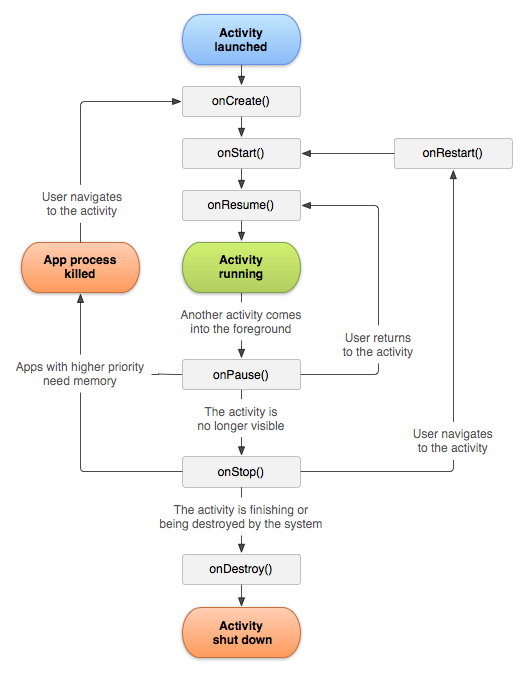
\includegraphics[width=350pt]{ActivityLife}\\
    \caption{Activity Life-cycle \cite{androidlife}} \label{Figure: Activity Life-cycle}
\end{figure}

\newpage

\section{Putting InforMe@Dublin Application on Google Play}
The informe app is signed with the author's credentials so that no intellectual information can be stolen or the application cannot be deconstructed by an unauthorised person to get the property of the developer. By uploading the application for reproduction on the Google play store the developer of informe had to gain the necessary SHA-1 encryption keys which were produced by the NSA used as a cryptographic hash function. The related encryption key creates a 160 bit or 20-byte hash value or also known as a message digest. 

\par The SHA-1 keys are needed to provide the related API keys on which are necessary for the usage of Google Maps as well as the OAuth used for the signing in of users authenticating with their Gmail account.
\newline
\textit{"C:\textbackslash Program Files (x86)\textbackslash Java\textbackslash jdk1.8.0\textunderscore 65 \textbackslash bin$>$ keytool -list -v -keystore "C:\textbackslash Users\textbackslash Adam O'Connor\textbackslash keyforInforMe\textbackslash InforMe@Dublin.jks" -alias     alias\textunderscore name -storepass password -keypass password"}

\begin{figure}[htbp]
    \center 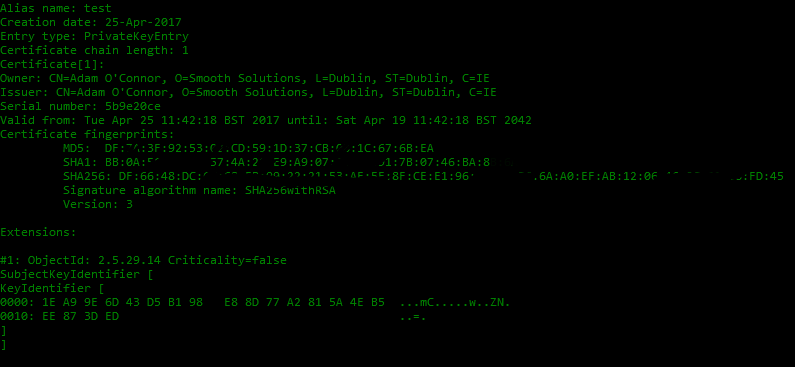
\includegraphics[width=450pt]{Hashkeys}\\
    \caption{Crypt Key Screenshot} \label{Figure: Crypt Key Screenshot}
\end{figure}

To obtain the SHA-1 key used in the generated signed APK the above console command is needed in order to retrieve the key which the developer needs to add to the Firebase database and OAuth 2 in both the Firebase console and Google API console. The Generated key store used to sign the application is needed to retrieve the SHA key. 

\section{A Way of allocating Permissions}
With regards to the new permissions that are now needed by applications to run on Android applications, a code listing was provided by the developer below. The new permissions were introduced by the Android development team with the release of Android marshmallow instead of users accepting terms of the downloaded application from the Google play store, and users would need to accept these permissions when needed throughout the use of such an application with are requested one by one. The developer has to call each request manually which is below.
\begin{lstlisting}[style=myCustomMatlabStyle, basicstyle=\small, breaklines, caption=Permissions Example,captionpos=b] 
 // check permission request of 99
 public static final int MY_PERMISSIONS_REQUEST_LOCATION = 99;
 
 /**
 * used to check the location permission
 * @return
 * dialog if user has not set permissions
 */
 public boolean checkLocationPermission() {
     if (ContextCompat.checkSelfPermission(this,
     Manifest.permission.ACCESS_FINE_LOCATION)
     != PackageManager.PERMISSION_GRANTED) {
     
         // Should we show an explanation?
         if (ActivityCompat.shouldShowRequestPermissionRationale(this,
         Manifest.permission.ACCESS_FINE_LOCATION)) {
         
             // Show an explanation to the user *asynchronously* -- don't block
             // this thread waiting for the user's response! After the user
             // sees the explanation, try again to request the permission.
             
             //Prompt the user once explanation has been shown
             //(just doing it here for now, note that with this code, no explanation is shown)
             ActivityCompat.requestPermissions(this,
             new String[]{Manifest.permission.ACCESS_FINE_LOCATION},
             MY_PERMISSIONS_REQUEST_LOCATION);
         
         
         } else {
             // No explanation needed, we can request the permission.
             ActivityCompat.requestPermissions(this,
             new String[]{Manifest.permission.ACCESS_FINE_LOCATION},
             MY_PERMISSIONS_REQUEST_LOCATION);
         }
             return false;
     } else {
         return true;
     }
 }
\end{lstlisting}
\par
The above code is used in conjunction with the requesting of the specific location permission of the device on which the app has been downloaded and opened. The location dialogue is the first permission on which would be shown to the user if the permission has not been set then the user cannot explicitly continue using the application. The dialogue module would simply keep showing until the user agrees to accept the location permissions. In conjunction with the checking location permissions method, an OnRequestPermissionsResult method is also used for the retrieval of such a permission request. The following method checks if the specific user has chosen to allow the app to receive the location of that app.
\newline
\begin{lstlisting}[style=myCustomMatlabStyle, basicstyle=\small, breaklines, caption=Permissions Request Example,captionpos=b] 
 /**
 *
 * @param requestCode
 * start to see if user connected
 * @param permissions
 * permissions which are needed for the application
 * @param grantResults
 * if the user has granted access to sensors.
 */
 @Override
 public void onRequestPermissionsResult(int requestCode,
 String permissions[], int[] grantResults) {
     switch (requestCode) {
         case MY_PERMISSIONS_REQUEST_LOCATION: {
             // If request is cancelled, the result arrays are empty.
             if (grantResults.length > 0
             && grantResults[0] == PackageManager.PERMISSION_GRANTED) {
             
                 // permission was granted, yay! Do the
                 // location-related task you need to do.
                 if (ContextCompat.checkSelfPermission(this,
                 Manifest.permission.ACCESS_FINE_LOCATION)
                 == PackageManager.PERMISSION_GRANTED) {
                 
                 }
         
            } else {
         
                 // permission denied, boo! Disable the
                 // functionality that depends on this permission.
                 checkLocationPermission();
             }
             return;
         }
         
         // other 'case' lines to check for other
         // permissions this app might request
     }
 }
\end{lstlisting}

\section{Utilising Firebase's Auth method}
Regarding the Firebase Auth method on which includes a user management system. With the following in mind, the developer can compare some basic data against the Firebase Auth users. Utilising the following method allows the developer to offer multiple login methods such as email/password, Google, Facebook. The following lets users link their accounts into a single Firebase account. Using the Auth method provides pre-existing auth system so that the application can take advantage of Firebase's security rules which have been set by the developer.

\section{Logging into Cloud services}
The cloud service on which this application connects to is Firebase. Firebase controls the authentication between the application itself and allows the signed in person to retrieve information which is located in the database. The following code was used in coordinance with the authentication with the following application.
\par
Email/password authentication has functions to register new users as well as signing them back in once registered. Firebase auth also provides a method of signing a user out of the application all functions return promises on which the new user registration as well as creating a profile on the database automatically signs the user in. The login information of the app is saved and holds the signing in information of the user if they have not signed out.

\begin{lstlisting}[style=myCustomMatlabStyle, basicstyle=\small, breaklines, caption=Authentication Example,captionpos=b] 

 /**
 * used for the signing in of a user which has logged in
 * with their email address and password.
 * @param email
 * email address of the user which created an account.
 * @param password
 * password on which user wants to use.
 */
 private void signIn(String email, String password) {
     Log.d(TAG, "signIn:" + email);
     // validate the textfields user has filled in.
     if (!validateForm()) {
        return;
     }
 
     showProgressDialog();
 
     // start the authentication of the email address and password of the user.
     final Task<AuthResult> authResultTask = mAuth.signInWithEmailAndPassword(email, password)
     .addOnCompleteListener(this, new OnCompleteListener<AuthResult>() {
         @Override
         public void onComplete(@NonNull Task<AuthResult> task) {
             Log.d(TAG, "signInWithEmail:onComplete:" + task.isSuccessful());
         
             if(task.isSuccessful()) {
                checkUserExistsDatabaseOnReEnter();
             }
             
             // If the sign in fails displays a message to the user. If sign in succeeds
             // the auth state listener will be notified and logic to handle the
             // signed in user can be handled in the listener.
             if (!task.isSuccessful()) {
                 Log.w(TAG, "signInWithEmail:failed", task.getException());
                 Toast.makeText(EmailPasswordAuthentication.this, R.string.auth_failed,
                 Toast.LENGTH_SHORT).show();
                 mStatusTextView.setText(R.string.auth_failed);
             }
         
            hideProgressDialog();
         }
     });
 }
\end{lstlisting}

The above method concludes the sign in of the application using the user's email and password to gain access to the following application. While choosing the sign in button after the user has entered their credentials the email and password will be used together with the use of Firebase Auth. The information is then sent to the Firebase project which is linked to the project utilising a google-services.json file of which is compromised of the client information of the app as well as the OAuth information which relates to the application. The google-services.json file will be added into the appendix in this chapter.
\par
With the following in mind, the  Google authentication of the users is used in the same way with some other methods used to map the OAuth 2 authentication together with the Google services API on which is automatically created in the Google console.  OAuth with web authentication is needed as it is a requirement of Android if the app is released on the Google play store as some instances are authenticated with the web authentication.
\newline

\begin{lstlisting}[style=myCustomMatlabStyle, basicstyle=\small, breaklines, caption=Google Authentication Example,captionpos=b] 
 // Configure Google Sign In
 GoogleSignInOptions gso = new GoogleSignInOptions.Builder(GoogleSignInOptions.DEFAULT_SIGN_IN)
     .requestIdToken(getString(R.string.default_web_client_id))//requesting the specific token the Google sign.
     .requestEmail() // requesting the email address of the user to sign in.
     .build();
 
 // creation of a Google API client for the connection of a Google token of the OAuth 2 API in the Google Console.
 mGoogleApiClient = new GoogleApiClient.Builder(this)
     .enableAutoManage(this, new GoogleApiClient.OnConnectionFailedListener() {
         @Override
         public void onConnectionFailed(@NonNull ConnectionResult connectionResult) {
         
         }
     })
     .addApi(Auth.GOOGLE_SIGN_IN_API, gso)// addtion of the Google sign in API and Google sign in options.
     .build();
 \end{lstlisting}

\section{Creation of User Preferences}
About the following section which utilises users preferences throughout the use of the InforMe@Dublin application. The developer will display some of the code of which is related to using user's preferences within an Android application environment the developer used preferences in informe by way of reusing the same activity but by producing different layouts to the user. Here is a following code listing of the preference method.

\begin{lstlisting}[style=myCustomMatlabStyle, basicstyle=\small, breaklines, caption=Preferences Example,captionpos=b] 

/**
* This fragment shows notification preferences only. It is used when the
* activity is showing a two-pane settings UI.
*/
@TargetApi(Build.VERSION_CODES.HONEYCOMB)
public static class NotificationPreferenceFragment extends PreferenceFragment {
    @Override
    public void onCreate(Bundle savedInstanceState) {
        super.onCreate(savedInstanceState);
        addPreferencesFromResource(R.xml.pref_notification);
        setHasOptionsMenu(true);
        
        // Bind the summaries of EditText/List/Dialog/Ringtone preferences
        // to their values. When their values change, their summaries are
        // updated to reflect the new value, per the Android Design
        // guidelines.
        
        bindPreferenceSummaryToValue(findPreference("notifications_new_message_ringtone"));
    }
}

\end{lstlisting}
With the code listing above on which was provided by the developer shows how the specific preferences are bound within the app.  As the user chooses to enter the settings activity, the following layout is provided upon request. Each of the two layout preference headers is used in conjunction with there specific layout files to produce to the user on request\newline
\begin{lstlisting}[style=myCustomMatlabStyle, basicstyle=\small, breaklines, caption=Preferences Header Layout Example,captionpos=b] 
<preference-headers xmlns:android="http://schemas.android.com/apk/res/android">

<!-- These settings headers are only used on tablets. -->

    // The following code snippet is used to produce the specific preference layout of Battery Saver
    <header
    android:fragment="adamoconnor.informe.Settings.SettingsActivity$DataSyncPreferenceFragment"
    android:icon="@drawable/batteryicon"
    android:title="Battery Saver" />

    // The following code snippet is used to produce the specific preference layout of Notification Preference.
    <header
    android:fragment="adamoconnor.informe.Settings.SettingsActivity$NotificationPreferenceFragment"
    android:icon="@drawable/ic_notifications_black_24dp"
    android:title="@string/pref_header_notifications" />

</preference-headers>
\end{lstlisting}
While the settings activity on which controls the following preference header's is extended to another class called AppCompatPreferenceActivity which itself extends PreferenceActivty is used to control and replace the view on which the user has chosen to use their personal preferences for the app. Users can choose the particular tone of the notification which will be sent to the user entering a Geofence. The other preferences the user of the app can choose to activate is the battery saver preference which will allow the screen of such a device to deactivate the screen display when the devices proximity sensor detects an object in front of it such as putting the device in the users pocket. This saves the battery life of the device which allows more time for exploring the InforMe@Dublin application.

\section{Retrieving of Google's Mapping System}
Within this following section of the implementation of the application is one of the most important tasks of the inforMe@Dublin application. Loading the map when the user chooses they want to display their location and to view the geofences in the area in which they are in. The map loading quickly and smoothly with regarding the users quality of play with the app is of utmost importance.Below is two code snippets of which are used to load the Google map onto the activity of the device asynchronously. The mapping resource is used as a fragment which is displayed over the event in question.
\begin{lstlisting}[style=myCustomMatlabStyle, basicstyle=\small, breaklines, caption=OnCreate Method Map Loading Example,captionpos=b] 

 mapFrag = (SupportMapFragment) getSupportFragmentManager().findFragmentById(map);
 mapFrag.getMapAsync(this);
 
\end{lstlisting}
Allowing for the integration of Google Maps into an Android application, a GoogleApiClient connection is needed on allowing the app to gain the necessary information to produce such a map fragment on the activity. The client of the ApiClient is initiated with the following code snippet below.
\begin{lstlisting}[style=myCustomMatlabStyle, basicstyle=\small, breaklines, caption=buildGoogleApiClient Code Snippet,captionpos=b] 

  /**
  * call the api client needed to retrieve information.
  * from google such as maps and the location API.
  */
  protected synchronized void buildGoogleApiClient() {
      mGoogleApiClient = new GoogleApiClient.Builder(this)
          .addConnectionCallbacks(this)
          .addOnConnectionFailedListener(this)
          .addApi(LocationServices.API)
          .build();
      mGoogleApiClient.connect();
  
  }

\end{lstlisting}
While loading the map fragment which is used in the InforMe@Dublin application to set specific UI components within the application, the developer can choose whether to show specific items within the map fragment. Within this section of the implementation, the developer has chosen to disable certain settings which then enables developer's to add their buttons or UI components which are then shown on the app. Within the section which enables certain UI components, the map type can be distinguished with layouts such as:
\begin{lstlisting}[style=myCustomMatlabStyle, basicstyle=\small, breaklines, caption=Map Types,captionpos=b] 

    mMap.setMapType(GoogleMap.MAP_TYPE_NORMAL);
    mMap.setMapType(GoogleMap.MAP_TYPE_SATELLITE);
    mMap.setMapType(GoogleMap.MAP_TYPE_TERRAIN); 
    mMap.setMapType(GoogleMap.MAP_TYPE_HYBRID);
\end{lstlisting}
Within the next code, listing below is how the map is asynchronously loaded within the application. The onMapReady method is called automatically when the actual map fragment is called upon.
\begin{lstlisting}[style=myCustomMatlabStyle, basicstyle=\small, breaklines, caption=Building the Map,captionpos=b] 

/**
* creating the map on the creation of the activity.
* set each of the UI components of the map, such as
* compass, etc.
* @param googleMap
* pass the map on which is being shown on the activity.
*/
@Override
public void onMapReady(GoogleMap googleMap) {

    mGoogleMap = googleMap;
    // type of map needed to display.
    mGoogleMap.setMapType(GoogleMap.MAP_TYPE_HYBRID);
    
    UiSettings uiSettings = googleMap.getUiSettings();
    uiSettings.setAllGesturesEnabled(true);
    uiSettings.setCompassEnabled(true);
    uiSettings.setMyLocationButtonEnabled(false);
    uiSettings.setMapToolbarEnabled(true);
    uiSettings.setZoomControlsEnabled(false);
    googleMap.setTrafficEnabled(false);
    
    //Initialize Google Play Services
    if (Build.VERSION.SDK_INT >= Build.VERSION_CODES.M) {
        if (ContextCompat.checkSelfPermission(this,
        Manifest.permission.ACCESS_FINE_LOCATION)
        == PackageManager.PERMISSION_GRANTED) {
            buildGoogleApiClient();
            mGoogleMap.setMyLocationEnabled(true);
        }
    } else {
        buildGoogleApiClient();
        mGoogleMap.setMyLocationEnabled(true);
    }
}

\end{lstlisting}

\section{Attaining Clients Correlative Location}
Regarding the location manager of which is needed to gain access to the location of the device is as follows on Acquiring the location manager of the device in question is not done by instantiating a LocationManager directly but by rather requesting an instance from the device by calling the following method getSystemService(Context.LOCATION\textunderscore SERVICE) which returns a new handler regarding a new LocationManager instance. While retrieving the user's location of the device permissions are needed to gain an accurate reading. With the following in mind, it is advised on using the GPS module together with an internet connection, With the application as follows an internet connection is needed by the user to use the app.
\begin{lstlisting}[style=myCustomMatlabStyle, basicstyle=\small, breaklines, caption=Location Request Settings,captionpos=b]

 /**
 * when requesting location, needs interval set and what accuracy
 * the developer wants to achieve.
 */
 protected void createLocationRequest() {
     
     mLocationRequest = new LocationRequest();
     mLocationRequest.setInterval(3000);
     mLocationRequest.setFastestInterval(5000);
     mLocationRequest.setPriority(LocationRequest.PRIORITY_HIGH_ACCURACY);
     
     LocationSettingsRequest.Builder builder = new LocationSettingsRequest.Builder()
     .addLocationRequest(mLocationRequest);
     
     mLocationSettingsRequest = builder.build();
 }
\end{lstlisting}

\par
The code snippet above provides a reference to the location gathering of the user's device on connecting to the following activity on which the method has placed the setting of the interval with regards to the updating of the current position every couple of seconds.
\begin{lstlisting}[style=myCustomMatlabStyle, basicstyle=\small, breaklines, caption=OnConnected Location updates,captionpos=b]

/**
* call to location updates on when the device changes
* coordinates, it is then updated on the map.
* @param bundle
* the information of the activity.
*/
@Override
public void onConnected(Bundle bundle) {
    
    if (ContextCompat.checkSelfPermission(this,
    Manifest.permission.ACCESS_FINE_LOCATION)
    == PackageManager.PERMISSION_GRANTED) {
        createLocationRequest();
        LocationServices.FusedLocationApi.requestLocationUpdates(mGoogleApiClient, mLocationRequest, this);
    }
}
\end{lstlisting}

\section{Finding the Corresponding Positions of Historic areas}
With regards to retrieving the geofences which are needed for the population of the UI components such as drawing a circle of the Geofence radius and the marker which is needed to see if the device has entered the Geofence in question. The snippet of code which is below shows the reference to the Firebase database which is then needed to retrieve a reference to the child nominator. The data on which is retrieved from the data snapshot is then split up and added into a HashMap.

\begin{lstlisting}[style=myCustomMatlabStyle, basicstyle=\small, breaklines, caption=Reteriving text Information of Monument,captionpos=b]

 /**
 * creation of new firebase reference which populates an array of the specific,
 * populates with the specific name of the area and the coordinates
 */
 DatabaseReference database = FirebaseDatabase.getInstance().getReference();
 final DatabaseReference myRef = database.child("geofences").child(town.toLowerCase());
 myRef.addListenerForSingleValueEvent(new ValueEventListener() {
     @Override
     public void onDataChange(DataSnapshot alerts) {
         
         for (DataSnapshot alert : alerts.getChildren()) {
             String myLandmarks = alert.getValue().toString();
             //splitted name | long | lat
             String[] splited = myLandmarks.split("\\|");
             // send to the package com.example.adamoconnor.test02maps.LoginAndRegister; Constants Landmarks Hashmap.
             LANDMARKS.put(splited[0], new LatLng(Double.parseDouble(splited[1]), Double.parseDouble(splited[2])));
         }
     }
     @Override
     public void onCancelled(DatabaseError databaseError) {
         
     }
 });
 \end{lstlisting}
 \par
 While the code above retrieves the Geofences and populates each of the historical places into a HashMap, the MapsActiviy is used in conjunction which displays each of these monuments coordinates on the map fragment. The snippet below is how these Geofences are populated. Keep in mind of which a reference of an ArrayList is then added which is populated with the information of the Landmarks Hashmap. The ArrayList in this instance is needed to see when the user's device in question is within the Geofence radius which in this case is 50 meters.
 
\begin{lstlisting}[style=myCustomMatlabStyle, basicstyle=\small, breaklines, caption=Displaying of Geofences,captionpos=b]
 
/*
* used for the loading of all geofences which where called from firebase when
* the user has signed in.
*/
for (Map.Entry<String, LatLng> entry : adamoconnor.informe.MapsAndGeofencing.Constants.LANDMARKS.entrySet()) {
      
      // creation of the geofence colour and border colour.
     // setting of each specific geofence.
      CircleOptions circleOptions = new CircleOptions()
           .center(new LatLng(entry.getValue().latitude,entry.getValue().longitude))
           .strokeColor(Color.argb(50, 70,70,70))
           .fillColor(getResources().getColor(R.color.Geofence))
           .radius(50);
      mGoogleMap.addCircle( circleOptions );
      
      //Place current location marker
      LatLng geo = new LatLng(entry.getValue().latitude,entry.getValue().longitude);
      MarkerOptions markerOptions = new MarkerOptions();
       markerOptions.position(geo);
       markerOptions.title(entry.getKey());
       markerOptions.icon(BitmapDescriptorFactory.fromResource(R.drawable.informe));//BitmapDescriptorFactory.defaultMarker(BitmapDescriptorFactory.HUE_MAGENTA)
      
      //adding marker to each geofence.
      mGeofenceMarker = mGoogleMap.addMarker(markerOptions);
      
      // add each to the geofence array list with the lat and long as well as the radius in meters.
      mGeofenceList.add(new Geofence.Builder()
           .setRequestId(entry.getKey())
           .setCircularRegion(
           entry.getValue().latitude,
           entry.getValue().longitude,
           adamoconnor.informe.MapsAndGeofencing.Constants.GEOFENCE_RADIUS_IN_METERS)
           .setExpirationDuration(adamoconnor.informe.MapsAndGeofencing.Constants.GEOFENCE_EXPIRATION_IN_MILLISECONDS)
           .setTransitionTypes(Geofence.GEOFENCE_TRANSITION_ENTER |
           Geofence.GEOFENCE_TRANSITION_EXIT)
           .build());
}
\end{lstlisting}
\par
Concerning the above code located in listing 6.14. The reader can then understand on how each geofence is loaded and then decoded into its specific geo-location. Each location is allocated a distinguishable marker from the Informe application with this in mind on selecting the marker of the area displays the name of the historical monument in question. The user can toggle to view these markers which open an option on getting directions of a monument of their choosing. Selecting this option will open up Google maps with the travel time etc. of the location.

\section{A Look at the Geofencing Notification Service}
When a user's device has received a location or the location has changed the developer has created a method to which calls the Geofencing request to see whether the user has entered that specific geofence on initiation. The following method is called in the code listing below.
\begin{lstlisting}[style=myCustomMatlabStyle, basicstyle=\small, breaklines, caption=Population of Geofences,captionpos=b]

/**
* used to see if user has entered a geofence.
*/
public void PopulateGeofences() {
    if (!mGoogleApiClient.isConnected()) {
        Toast.makeText(this, "Google API Client not connected!", Toast.LENGTH_SHORT).show();
        return;
    }
    
    try {
        LocationServices.GeofencingApi.addGeofences(
        mGoogleApiClient,
        getGeofencingRequest(),
        getGeofencePendingIntent()
        ).setResultCallback(this); // Result processed in onResult().
    } catch (SecurityException securityException) {
        // Catch exception generated if the app does not use ACCESS_FINE_LOCATION permission.
    }
}
\end{lstlisting}

While reading through the different implementations of some of the most important parts of the application the following section represents how notifications are initiated when a device enters such a location. While each of the HashMaps Geofences is loaded, they are also added to an ArrayList and sent to the GeofencingRequest method which allows for the checking if the device enters a geofence.

\begin{lstlisting}[style=myCustomMatlabStyle, basicstyle=\small, breaklines, caption=Geofence Request and Pending Intent,captionpos=b]

/**
* get the geofence which is requested.
* @return
* to the pending intent.
*/
private GeofencingRequest getGeofencingRequest() {
    GeofencingRequest.Builder builder = new GeofencingRequest.Builder();
    builder.setInitialTrigger(GeofencingRequest.INITIAL_TRIGGER_ENTER);
    builder.addGeofences(mGeofenceList);
    return builder.build();
}

/**
* sending the notification to the user when geofence is entered.
* @return
*/
private PendingIntent getGeofencePendingIntent() {
    
    Log.d(TAG, "Geo fence pending intent");
    Intent intent = new Intent(this, GeofenceTransitionsIntentService.class);
    // We use FLAG_UPDATE_CURRENT so that we get the same pending intent back when calling addgeoFences()
    
    return PendingIntent.getService(this, 0, intent, PendingIntent.FLAG_UPDATE_CURRENT);
}
\end{lstlisting}

\section{Retrieving Information of Historical Monuments}
With regards to the implementation of loading the historical monuments within the application was coded as follows by the developer of the following project. While the user of the device enters a geofence location with the intention of a notification looming on entering the geofence, that is produced with a pending intent. When a pending intent has then initiated a notification is then sent to the user's device of which is retrieved by the MapsActivity. If the user is using the app at the time or the user can simply choose to click the notification and be sent to the information activity which will show the subsequent history of that location. With that in mind, the name of the monument name is passed to a set variable which is located in the Place class.

\begin{lstlisting}[style=myCustomMatlabStyle, basicstyle=\small, breaklines, caption=Loading Information of Monuments,captionpos=b]

 /**
 * load the specific data of the historic information
 * this method retrieves the text for the activity
 * with a reference to load images.
 */
 private void LoadData() {
     
     //reference to Firebase database.
     DatabaseReference myRef = database.child("ruin");
     myRef.addValueEventListener(new ValueEventListener() {
         @Override
         public void onDataChange(DataSnapshot dataSnapshot) {
             
             //reference to load images method.
             informationImages();
             
             try {
                 
                 String info = (dataSnapshot.child(getMonumentName().trim()).getValue().toString());
                 title.setText(monumentName.trim());
                 String regex = "\\[|\\]";
                 info = info.replaceAll(regex, "");
                 information.setText(info);
                 
             } catch(NullPointerException ex) {
             LoadData();
         }
         
     }
     
     @Override
     public void onCancelled(DatabaseError databaseError) {}
     
 });
}
\end{lstlisting}
\par
With hence to the code located above the reader can see where the developer has provided a reference to the tree node of the Firebase database of which the following activity must have access to.  After the reference connection has been completed the monument name of the intent is passed to the informationFrontFragment on which populates the information text field with the appropriate text allocated in the Firebase database. When the following information has been retrieved the developer then has to perform a regex to remove certain elements from the text on which the Firebase database add's brackets to multiple lines of text.
\par
With regards to retrieving the images of which are related to a monument is compromised in a similar way to retrieving the child node of the parent in the database. For the population of each of the images, they are then compiled into a hash map and given a unique identity which is provided by a counter. These image URLs which are allocated by their monuments name and value of which were retrieved are then added onto a sliderLayout which will be changed every three seconds. The following code listing - 6.18 represents the loading of these images from the HashMap.

\begin{lstlisting}[style=myCustomMatlabStyle, basicstyle=\small, breaklines, caption=Loading Images on InformationFrontActivity,captionpos=b]

 Hash_file_maps = new HashMap<>();
 
 // load the images add numbers.
 int count = 1;
 for(DataSnapshot alert : alerts.getChildren()) {
     // pass the monument name
     Hash_file_maps.put(monumentName.trim()+", "+count, alert.getValue().toString());
     count++;
 }
 
 // add the images to the slider.
 for(String name : Hash_file_maps.keySet()) {
     
     TextSliderView textSliderView = new TextSliderView(getContext());
     
     textSliderView
         .description(name)
         .image(Hash_file_maps.get(name))
         .setScaleType(BaseSliderView.ScaleType.Fit)
         .setOnSliderClickListener(InformationFrontFragment.this);
         
     textSliderView.bundle(new Bundle());
     
     textSliderView.getBundle()
         .putString("extra",name);
     sliderLayout.addSlider(textSliderView);
     
 }
\end{lstlisting}

\section{Storage of Data}
With regards to the storing of the InforMe@Dublin information as well as each specific geofence location that is to be loaded onto a mapping application. Firebase is the answer to all of the questions while utilising the power of Firebase with regards to the security and anonymity of each specific user's data with reference to the users passwords and email address's all of these privacy issues are dealt with the Firebase console the developer doesnt have access to any password of which patrons of the application has set these are only reference by the unique identity key.

While the JSON data is added into the Firebase database the image below is what the InforMe@Dublin database actually look's like while the methods above show the retrieval of information from the database. Each line of these strings are associated with a corresponding parent.

\begin{figure}[htpb]
	\centering
	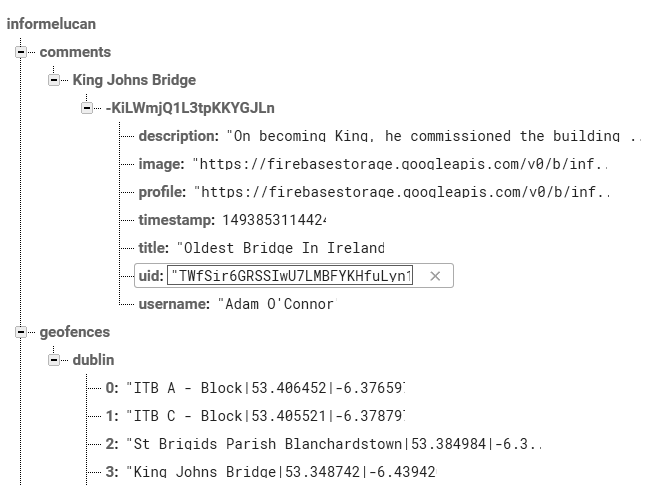
\includegraphics[width=300pt]{database1}\\
	\caption{Firebase Database} \label{Figure: Firebase Database}
	
	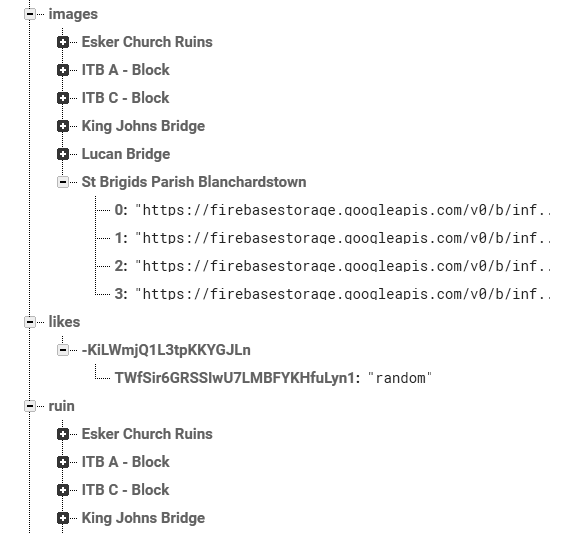
\includegraphics[width=300pt]{database2}\\
	\caption{Firebase Database} \label{Figure: Firebase Database}
\end{figure}

\newpage

\section{Summary of the Chapter}
Regarding the following chapter, the developer of the InforMe@Dublin Android application displayed and discussed some of the more important methods of the classes in the app. Most of the listings which are referenced by a unique identification number, regarding each of the methods and code snippets referenced above in the chapter the full code of the following application is supplied within the following thesis.

\chapter{Testing and Evaluation}

\section{Description of the Chapter}
Regarding the following chapter, the developer will provide the testing of the application on which will prohibit errors running throughout at specific points and within the application. Some visual testing of the app has been conducted within which some guests were allowed to test upon the release of it to the Google play store. The smoothness of the application and latency issues, as well as any other problems which may have been discovered on completing such an app, would be delivered and results published.Testing any application which is due to be release needs vigorous testing some of the most tests related to application development are functional testing, usability testing, security testing as well as a not so complicated method of visually assessing the code of which was written. For an application to be release, a mobile application must be able to satisfy each of these testing methods.
\section{Functional Correctness}
\textbf{\textit{Does the functionality of the following project meet the standards of what the project is intended for?}}
\newline
The answer to the question above is yes, the project functions above the expectation of the developer which is why the developer has chosen to publish the application on the Google Play Store. All parts of the program perform well and do what the developer has intended the app in question to do. 
\par
Each action of which a user will choose will do what it is supposed to do and will not receive any unknown errors unless something drastic or problematic is wrong with a device on which intends to use or install the following app. The graphical display is easily understood but could use a how-to tutorial after the creation of an account within the app for the not so experienced users.
\par
With the exception of accepting permission's on the app as well as entering the user's details if these have not been entered an error on the text field would be shown graphically to the user.

\section{Loading of the Application}
Regarding the fast usability of the InforMe@Dublin application with regards to latency related issues, the following application has none of this kind. While the developer was coding the loading up of the application and authentication, the user just has to wait until the progress dialogue completes which means the user is in the process of being logged into the app which helps as a user is not trying to access certain UI elements while a long process is being completed. Overall the application has a smooth feel to it with no issues being related to latency issues. This may happen on some device with a low amount of ram available to the device.

\section{Loading of the Map}
While the map loads on the mobile device a camera animation is performed this allow's for a nice smooth feel to the user's location. Utilising these actions on the device leave's users with a great feel while accessing the app as it seems good quality overall with regards to scoping out the location of the device. Only errors will occur if the device cannot receive the geofences on which need to be received from the Firebase database.

\section{Loading of the Information}
Concerning loading the information of each specific Geo-lateral location while the developer was coding the application some latency issues were happening with regards to the API the developer was using which allows for the information to be justified and evenly spaced. Using the following class which is available to integrate with any Android project can be found on Github by bluejamesbond called TextJustify-Android. The following class although nice in styling provides text being loaded only at certain times which means that the development of this class has not been completed. With that in mind, the developer had found an alternative which is called JustifiedTextView by Navabi together while using the following class and using the Picasso API provided the needed processing power for the app not to become sluggish or not to display certain aspects of the activity.
 

\section{Efficiency of the Application}
The efficiency of the project as a whole is that is above that of what the developer expected. Considering the number of connections that could be going on at the same time regarding accessing the Firebase database and retrieving the authenticity of the users with their unique identity tags as well as processing each of the geo-locations which on opening the map activity is loaded asynchronously in such a fast and smooth manner. The efficiency of the app is produced by using worker threads in conjunction with the UI-thread of the Android device on which the application is installed this allows for multiple processes to be done simultaneously. When developing the application, the developer noticed some latency and concurrency issues while developing such an application concerning the loading of images which was done by using Picasso which allows for the downloading of images smoothly and in a synchronous type fashion, Picasso uses Automatic memory and disk caching for all images loaded with the following API. Also, async threads are also used to create a smooth feel while a user is utilising such an app. 
\par
While using the application, the device can use the mobile's data on which is fast enough for utilising an application of the following standard. Visiting different monuments within the application allows for the caching of these images and information this saves on the data usage of the application, The developer tested this by using the application over a period of time and of which the application only used 30mb of data.

\section{Usability of the Application}
A set of tasks were given to each user of the following application's quality and usability with regards to the testing of the application. The developer compiled a set of task for each user to complete. Testing of the application needed to be throughout as the developer did not want users of the application to be hit with multiple app crashes. Also, the application needed to be easily enough to use as people of all ages could use the InforMe@Dublin app. Using the program should be easily read and perform as intended as the developer promised.

\section{Tasks on using the Application for a Tester}
\begin{enumerate}
\item Logging into the InforMe@Dublin app.
\item Creation of an Account.
\item Changing notification sounds.
\item Changing power saving option.
\item Toggle focusing on devices location.
\item Adding new geofences which will be sent to the developer.
\item Using the compass of the application.
\item Choosing a geofence marker on which users can get directions using Google Maps.
\item Entering a geofence to continue onto the information of a monument.
\item Choosing text-to-speech allowing the user to listen to the information of the monument.
\item Looking at users comments.
\item Liking users comments.
\item Adding comments.
\item Removing comments.
\item Updating comments.
\item Logging out of the application. 
\end{enumerate}
\section{Tester 01}
The followings testers background is as follows. Tester one's job title is that of a graphic designer who works within the mobile phone industry within Dublin city centre. The tester is 23 years old uses mobile phones every day and has a Samsung Galaxy 6S which boasts an astonishing number of high specifications such as a whopping 3GB of Ram. The tester downloaded and installed the InforMe@Dublin application on their device and a set of tasks where given.

\subsection{Graphic Display}
It is very professional looking. The layout is clear and informative. Very impressive for a student project.

\subsection{Usability}
I found the app user-friendly. Straight forward and easy to use. Anyone of any age would be able to navigate around the app successfully.

\subsection{Additional Comments}
Would love to see more locations. Keep up the good work

\section{Tester 02}
Tester two, the next tester is a male of 48 who's occupancy is a factory worker. Working for one of Ireland's most prestigious paint companies located in Celbridge but lives in Lucan Co.Dublin. The testers device is an Alcatel Idol 4, which is a budget mobile device. The tester downloaded and installed the InforMe@Dublin application on their device and a set of tasks where given.

\subsection{Graphic Display}
The display is quite nice. Overall there is a good feel to this app.

\subsection{Usability}
It works, the app does on what the developer intended it to do. I might even use it while going on walks to learn about our area.

\subsection{Additional Comments}
Best of luck in your future endeavours.

\section{Tester 03}
Tester three's background is of a professional fitness tutor working closely with the ncef and of which is the owner of their own business within the fitness sector. The device on which this tester has used the app on is a Sony Xperia XA. The tester downloaded and installed the InforMe@Dublin application on their device and a set of tasks where given.

\subsection{Graphic Display}
The Graphical display is a superb standard compared to other apps on the play store. I find this application to be very appealing.

\subsection{Usability}
The functionality of this app is great walking around and looking at different aspects of history really makes you think and realise of what little other people had compared to what is in the same location now. The feel of the layout is quite neat.

\subsection{Additional Comments}
I would like to wish the developer of InforMe@Dublin all the best with this app. As I see it going far into the future.

\subsection{Security Testing}
The following application InforMe@Dublin uses Firebase for authentication of each user of the application. While using their email and password or Google authentication, the user of the app must create an account on the app on which they must provide their name and profile image. On creation of an account, the user is then added to the Informe Firebase database. While the user has entered the app, a check is done on which compromises of finding the unique id of the applicant in the database, if no user is found then an account is needed to be created. While testing the application regarding the login of a user concerning email and password authentication works a treat as the developer can see the database updating with the user's credentials on login and creation of an account. With regards to Google authentication, while adding the following application onto the Google play store, the developer had to retrieve the SHA-1 key used for the app release. Each API used within the development of the app a Signing-certificate fingerprint or the SHA-1 is added to each API licence.

\section{Visual Testing}
Visual testing of the InforMe@Dublin application was used to verify that the program would work as intended by the developer. While developing different parts of the application, the author would run these specific parts to see if the following code would conduce with other parts of the project to produce the outcome on which the developer was trying to achieve. While running the application, the developer could then see if the standard was paired with the code of which was written. Other standards were also needed which included exception classes to allow for errors to generate with an exception. Each part of the InforMe@Dublin project was overseen by the following method of testing on which was the most efficient, cost-effective and non-time consuming for the developer at that specific time.
\par
While also using the following testing method with the following application be developed on an Android mobile device on which allowed for the developer to use the specific developers debugging tools of which showed the usage of the CPU. Using the application as well as the GPU renderings of the application regarding the graphics of which are needed or used within the app.
\section{Summary of Chapter}
Regarding the following chapter, the developer of the InforMe@Dublin Android application has discussed the different methods and problems of which arrived while completing the application. Different test methods used such as real user experience as well as using the developers own initiative in regards to which method does what and following the methodology of which was chosen by the developer. The selected methodology allows for only moving on from one correct coding function to another when it has been extensively validated. The next chapter in this thesis is about the future work which may be undertaken by the developer.


\chapter{Conclusions and Recommendations for Further Work}

\section{Summary and Main Conclusions}

Following the review of literature which is located in (Chapter 3), four main research questions were identified regarding the project as a whole.

\begin{enumerate}
    \item\textbf{\textit{Is there a need for an application like this on the marketplace?}}
    
    \item\textbf{\textit{Is there a way to save battery life while using GPS / Internet connection within an android application?}}
    
    \item\textbf{\textit{Will location services, and mobile internet take much battery or data?}} 
    
    \item\textbf{\textit{Will the APP provide a wiki type interface where visitors can add to the information about a historic site?}}
    
\end{enumerate}  

\subsection{Developments and Findings Relating to Research Objective 1}  
With regards to the following question on which the author is to provide an answer to is yes there is quite a market for this application. The developer of InforMe@Dublin has received many words of praise before even releasing an app of the following standard. Researching application's of this type and standard throughout the Google Play market are of non-existence the developer of which had released a small survey to the general public of Lucan as a pilot scheme on distinguishing if the idea of an application within its category would fit in with their need's. Utilising a survey website called Survey Monkey was used in the creation of the survey which was published to the people of Lucan.

\begin{figure}[htbp]
    \center 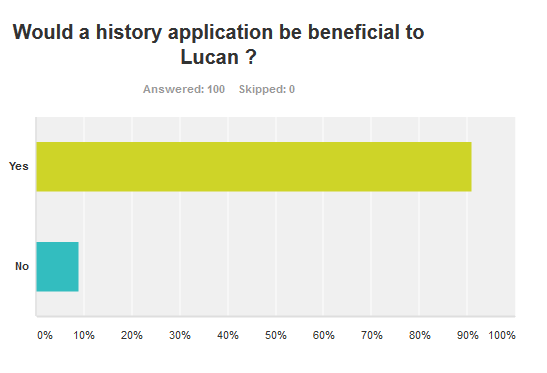
\includegraphics[width=350pt]{Lucan}\\
    \caption{Need for InforMe@Dublin} \label{Figure: Need for InforMe@Dublin}
\end{figure}

Regarding figure 9.1 the developer has shown one of the results on which were retrieved from the survey of which suggests that the people of Lucan would love to see an application of the following stature.

\begin{figure}[htbp]
    \center 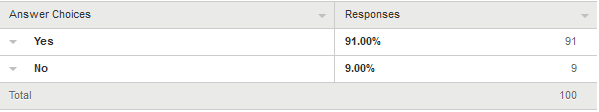
\includegraphics[width=350pt]{Lucanresponces}\\
    \caption{Number of Patrons who Completed Survey} \label{Figure: Number of Patrons who Completed Survey}
\end{figure}

The number of patrons who took part in the survey with relation to seeing if the InforMe@Dublin application was a good choice. 91 out of the 100 patrons who completed the survey said that they would be interested in such an application while nine said no. This could be that some of the patrons who took part in the survey were not actually from Dublin and may live in other area's or that the specific audience of which was targeted wasn't the best choice such as 15 - 19 year old's.

An application which is related to the InforMe@Dublin that the developer has found was produced for the telling of information of the 1916 rising located here in Dublin City Centre the app of which was developed by Failte Ireland. The Dublin Discovery Trails application is for the use of guided tours within the city centre itself which tells the story of Dublin over 1000 years. The app which use's devices location but stores all necessary files on the application itself and is only useful in Dublin city before going on these walks the application prompts user's to download a specific audio and image files which isn't much use if the patron is on the go.

\subsection{Developments and Findings Relating to Research Objective 2}
Regarding objective two which is related to the life of a battery while using location services as well as the internet connectivity. The battery life can be saved by using Google Play Services of which provide a battery manager of which is provided within the application to provide the best and most suitable power/accuracy ratio on gaining the location of an Android device.

The answer is yes. The battery life of an Android phone can be optimised by being smart with the development of the application. Breaking each part into specific smaller piece’s allowing threads to do individual tasks will help the life of the user’s battery, Also by using less service’s such as not calling all of the Google service’s packages will assist the battery life by using only a particular package. \cite{andBatt}

As the following application is to be used for educational purposes and doesn't ambit the need for adverts of which provides 75\% of application related battery drain. The following study was provided by Purdue University in partnership with Microsoft. These studies were concluded by looking at free application's located in the Google Play Store and the Apple store. As ad-serving provides its advertisers with valuable data from many patrons of many applications. In a nutshell advertiser's cover the cost of the application which is why it is delivered free to the user. The problem of these Ad-serving SDK's are that they are in fact poorly coded with regards to sending the information back to servers as well as the activity on the screen.\cite{admob} 

Also while using Firebase on which is incorporated within the Android application allows for the saving of some data on which has been loaded from the database this allows for the device to show this data which doesn't need to be parsed and downloaded again.

\subsection{Developments and Findings Relating to Research Objective 3}
While retrieving the location of a mobile device the following information was retrieved from a source which provides each of the location techniques, as well as the amount of power each of these, utilise while in use. This information was gathered when the author was researching different technologies that would be used or potentially used in the application.
\begin{table}[!ht]
    \centering
    \caption{Battery Usage of Positioning Techniques \cite{bareth2011energy}}
    \label{Battery Usage of Positioning Techniques}
    \begin{tabular}{@{}llrl@{}}
        \toprule
        \multicolumn{1}{c}{\textit{Technologies}} & \textit{Accuracy} & \textit{Precision} & \textit{Energy} \\ \midrule
        GPS & 10m & 95\% & 6.616Ws \\ \midrule
        WiFi & 50m & 90\% & 2.852Ws \\ \midrule
        Cellular-ID & 5km & 65\% & 1.013Ws \\ \bottomrule
    \end{tabular}
\end{table}

The following screen shot located in figure 9.3 was taken from the test device of which the InforMe@Dublin application was developed on. In the figure below shows how much data of which the application had consumed over the hour test. Below shows that on average the application does not exactly use that much data compared to other applications over an hour interval.

\begin{figure}[htbp]
    \center 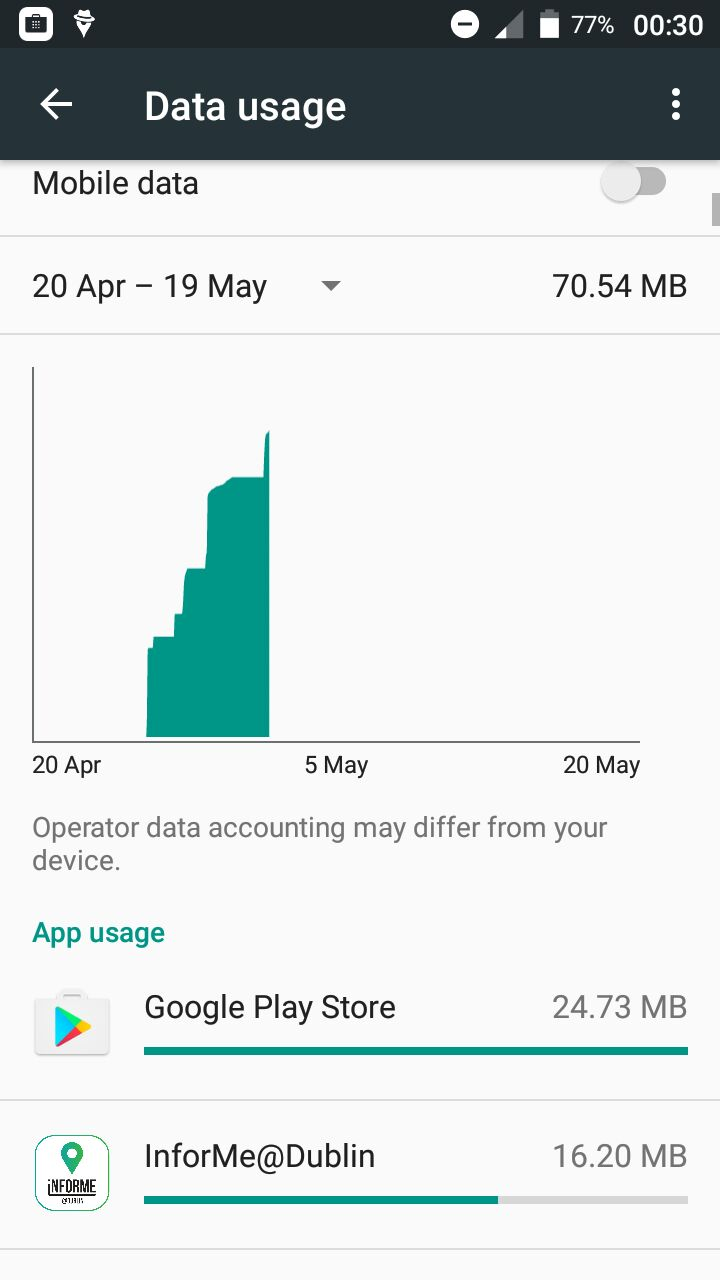
\includegraphics[width=150pt]{dataused}\\
    \caption{Data usage of InforMe@Dublin} \label{Figure: Data usage of InforMe@Dublin}
\end{figure}
\newpage

\subsection{Developments and Findings Relating to Research Objective 4}
During the development of such an application, the developer decided on introducing a different type Wiki feel to the application which allows the users to contribute to the information on such areas by posting different images of that area whether that being new or old images. While each patron has added their individual information of the area. Other users can then like posts of which have been created. Only that specific user who created the post can remove and update it on the application if they wish to re-visit the Geofence location. A Screen-shot of the applications wiki type feel is shown below in figure - 9.4

\begin{figure}[htbp]
    \center 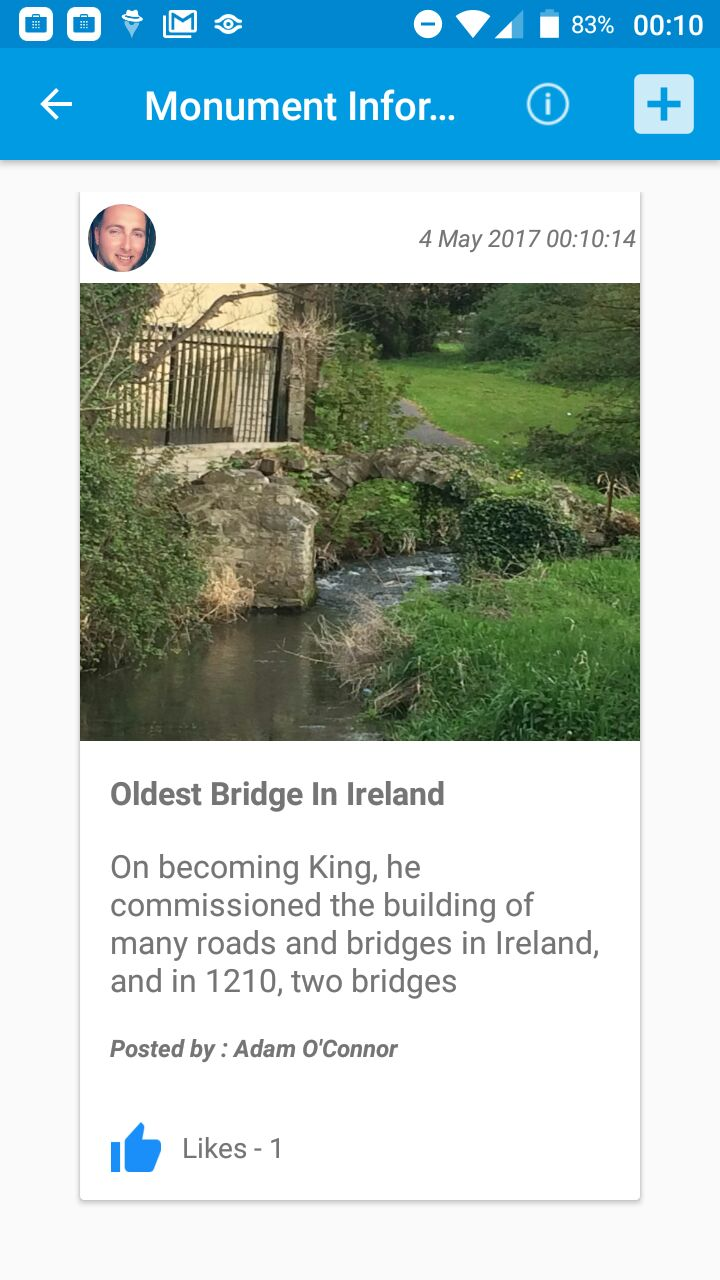
\includegraphics[width=150pt]{wikifeel}\\
    \caption{Wiki Type Activity} \label{Figure: Wiki Type Activity}
\end{figure}
\newpage

\section{Recommendations for Further Work}
With regards to the developer continuing with the development of the Android application InforMe@Dublin. The developer as follows thinks that the project as a whole is worthy of more development bringing the app to even more devices as it is only limited to Android Marshmallow devices and above. With the future of technology where it is today, there is a significant opportunity for providing an application to other users not just specifically to Dublin so the Informe app can be expanded and provided to people all over Ireland.

the following future work objectives can be completed.
\begin{enumerate}
    \item Providing more historical monuments to the application.
    \item Adding a new way of users to add a Geofence.
    \item Creation of specific profile pages of user's.
    \item Providing more cost effective ways on users using the application with a connection to the internet.
    \item Provide more power efficient code which allows users to explore more.
    \item Adding a how to page or tutorial on how to use the InforMe@Dublin application.
\end{enumerate}

\chapter{Personal Reflections}

Regarding the following project InforMe@Dublin, the developer has expressed Great enjoyment on creating an application of the following standard. The application was a joy on completing which allowed the developer to show the skills on which he has learnt over the past four years studying computer science at the Institute of Technology Blanchardstown. Regarding the skills needed for completing such an app of a high standard and the progressing to the release of an app which is the only one of its kind located in the Google play store. Some problems faced throughout the development of such an application where the concurrency issues of which related to the accessing of the Firebase database and populating the monument fields, Geofence locations and data on which other users have added. Some of these methods on which needed access to the database of which had to be slowed down on processing the data within the app. It was fun creating an app from scratch seeing a theory in the developers head into becoming a fully functional Android application. The developer would like to update the app into the distant future continually and updating the geofences of different area's but also to include a website on which geofence's can be added and updated as well as uploading the associated images.

\section{Fingal County Council Feedback}
Concerning sending the InforMe@Dublin application to Fingal county council, the developer received some feedback which was good news. The person who is an editor and project manager of Dublin.ie thought that the application was quite good considering it's a student project. On first installing the application the user had a problem with signing into the app which was a weird error considering the installation was tested on a few devices. Anthony Mc Guinness wished the developer all the best of luck on developing the InforMe@Dublin Android Application.

\section{Dublin City County Council Feedback}
Regarding receiving feedback from Dublin City Council, the developer was directed to the Mobile Device section, of which was notified of the application due to a contract that is between the council and their work mobiles they cannot install unknown applications. Because this application doesn't have enough recognition with regards to known security risk factors they cannot download these unknown applications even though the application is on the Google Play Store and passed all security screening. While the application uses the mobile's location and access to photographs and media files, it cannot be installed on their device hence forfeiting a contract of which they have made with the mobile provider. 
\chapter{Appendix A}

\section{InforMe@Dublin Screen Shots}
In the following section of the appendices, the developer has submitted screen shots of the InforMe@Dublin. Each page of the application is presented below just as an aid to the reader on understanding what the app presents to the users that download it from the Google Play Store.

\begin{figure}[!tbp]
	\centering
	\begin{minipage}[b]{0.4\textwidth}
		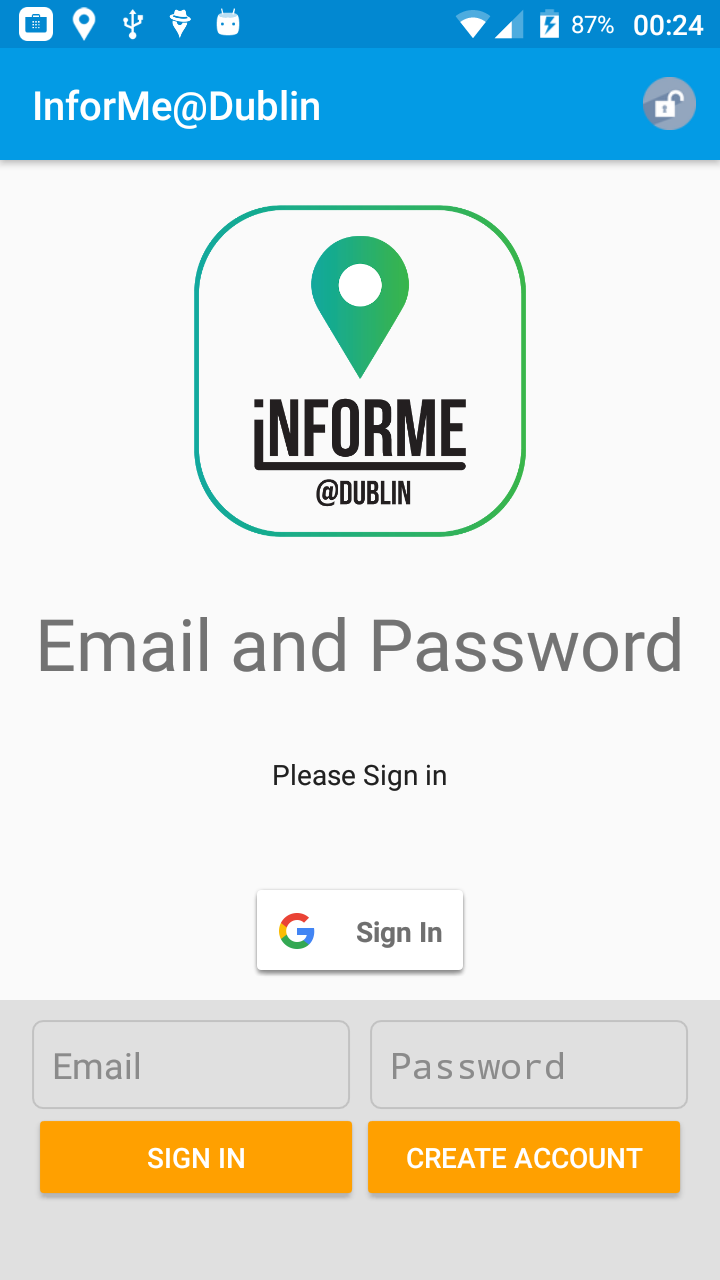
\includegraphics[width=150pt]{Login-Page}
		\caption{Login Page}
		\label{Figure: Login Page}
	\end{minipage}
	\hfill
	\begin{minipage}[b]{0.4\textwidth}
		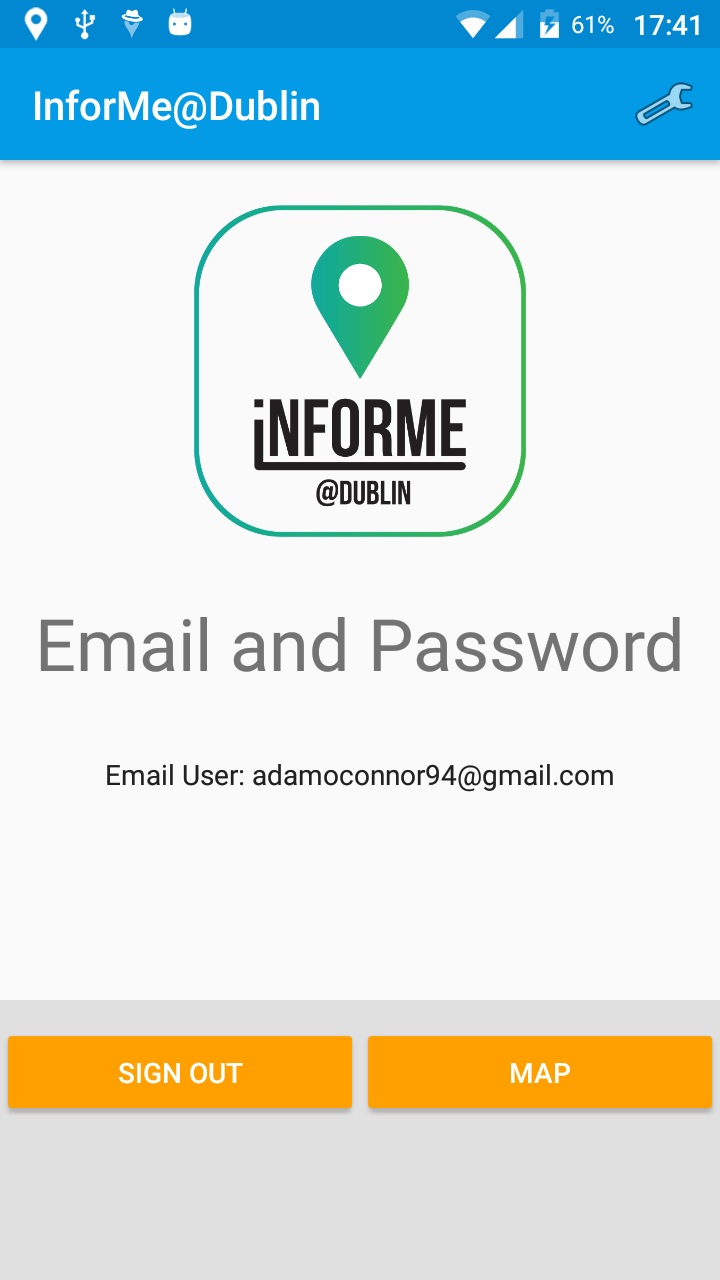
\includegraphics[width=150pt]{LoggedIn-Page}
		\caption{Logged in Page} 
		\label{Figure: Logged in Page}
	\end{minipage}
\end{figure}

\begin{figure}[!tbp]
	\centering
		\begin{minipage}[b]{0.4\textwidth}
			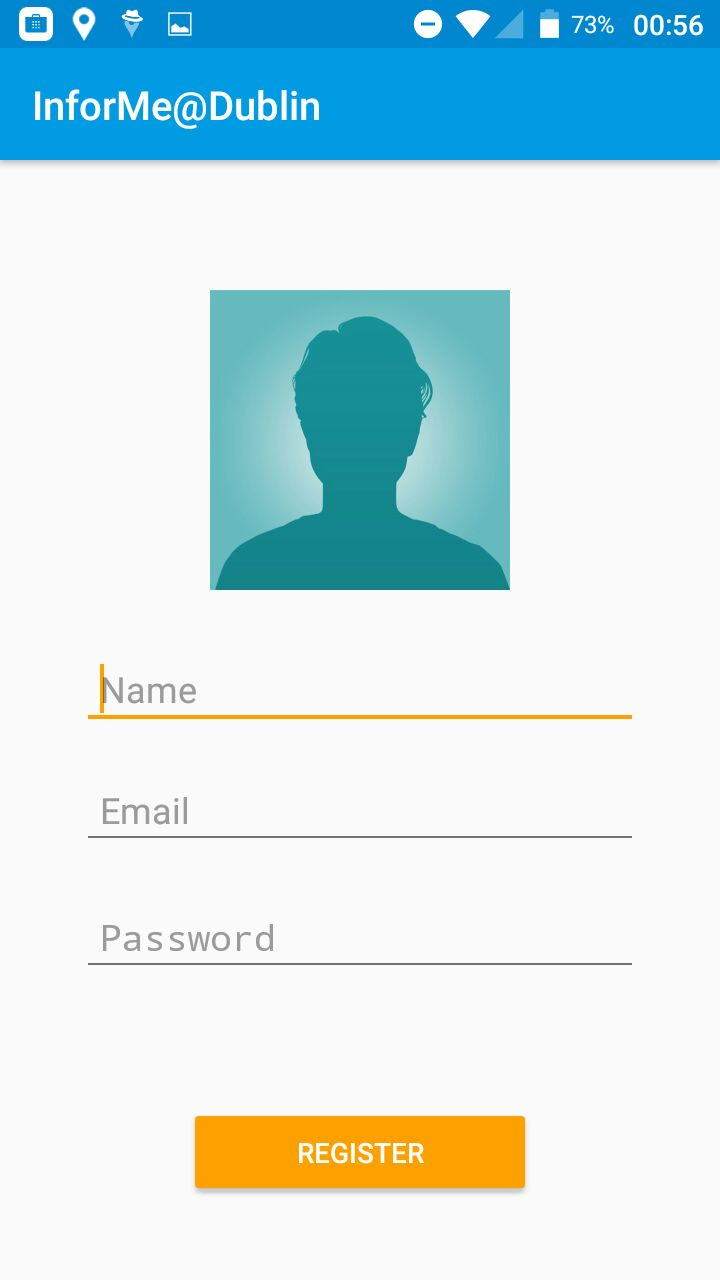
\includegraphics[width=150pt]{register}
			\caption{Register} 
			\label{Figure: Register}
		\end{minipage}
	\hfill
		\begin{minipage}[b]{0.4\textwidth}
			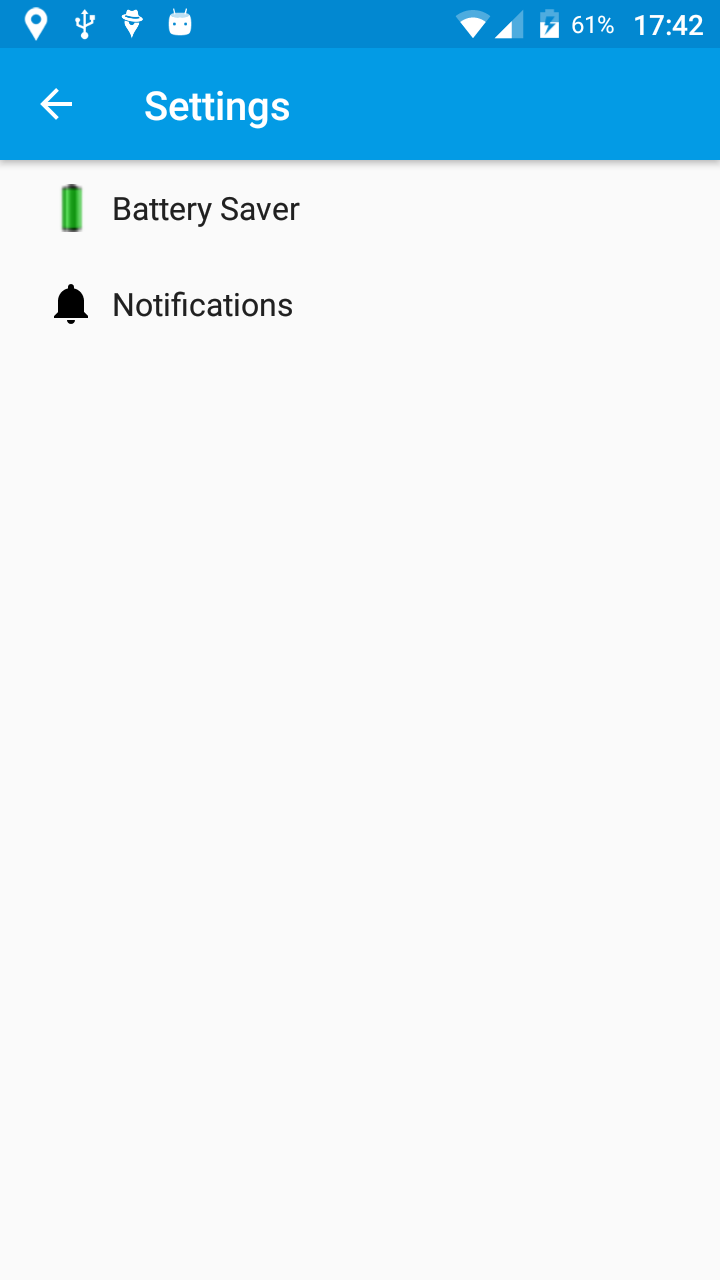
\includegraphics[width=150pt]{Settings-Preference}
			\caption{Settings Preference}
			\label{Figure: Settings Preference}
		\end{minipage}
\end{figure}
%%%%%%%%%%%%%%%%%%%%%%%%%%%%%%%%%%%%%%%%%%%%%%%%%%%%%%%%%%%%%%%
\begin{figure}[!tbp]
	\centering
	\begin{minipage}[b]{0.4\textwidth}
		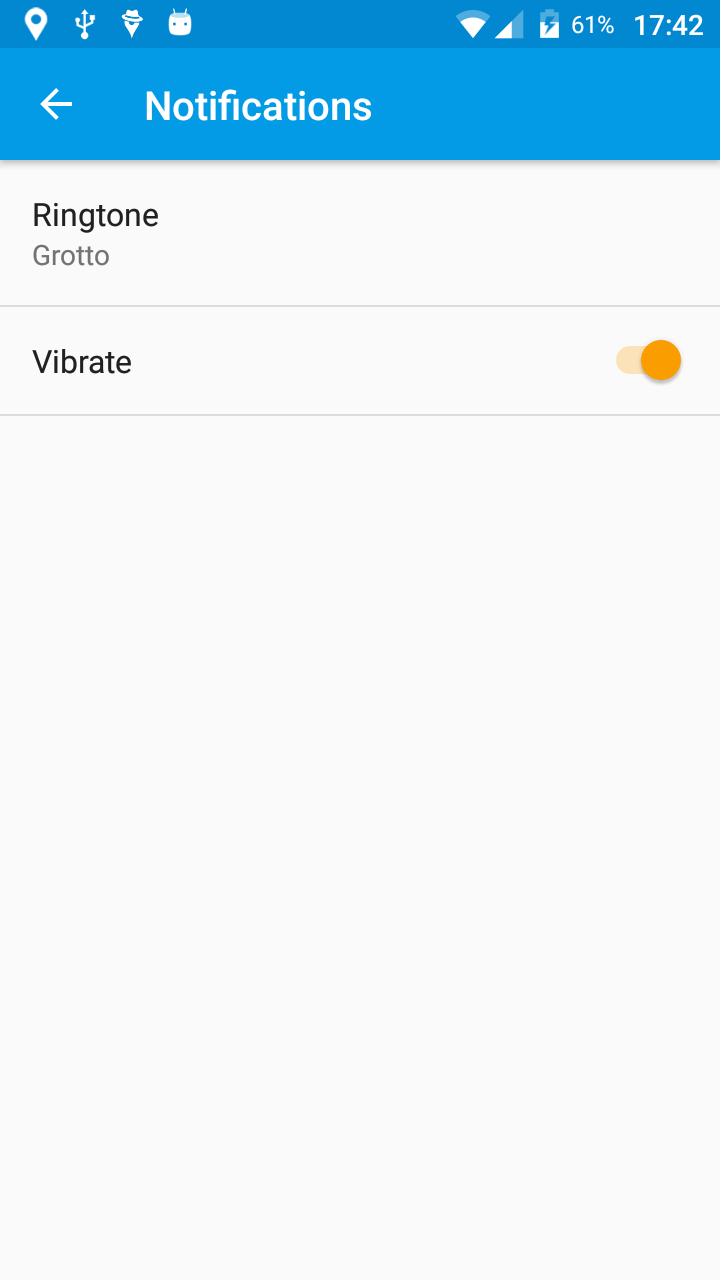
\includegraphics[width=150pt]{Notification-Settings}
		\caption{Notification Settings}
		\label{Figure: Notification Settings}
	\end{minipage}
	\hfill
	\begin{minipage}[b]{0.4\textwidth}
		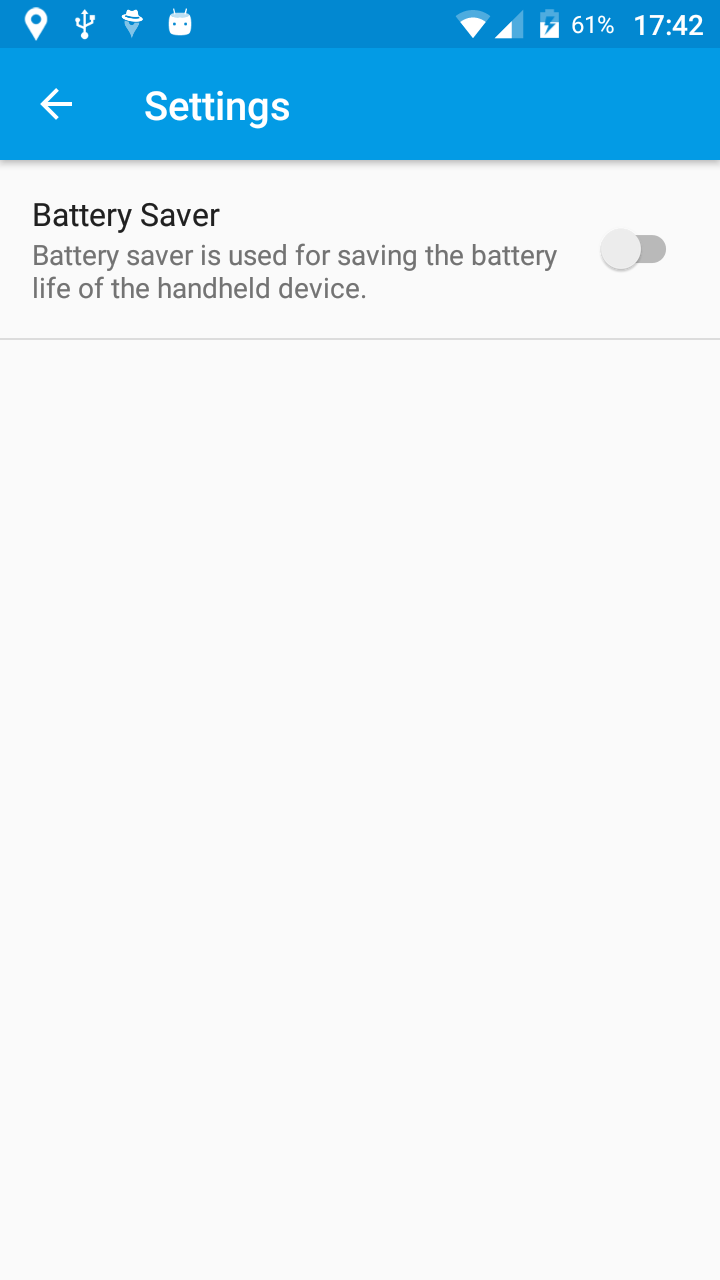
\includegraphics[width=150pt]{Battery-Settings}
		\caption{Battery Settings} 
		\label{Figure: Battery Settings}
	\end{minipage}
\end{figure}
%%%%%%%%%%%%%%%%%%%%%%%%%%%%%%%%%%%%%%%%%%%%%%%%%%%%%%%%%%%%%%%
\begin{figure}[!tbp]
	\centering
	\begin{minipage}[b]{0.4\textwidth}
		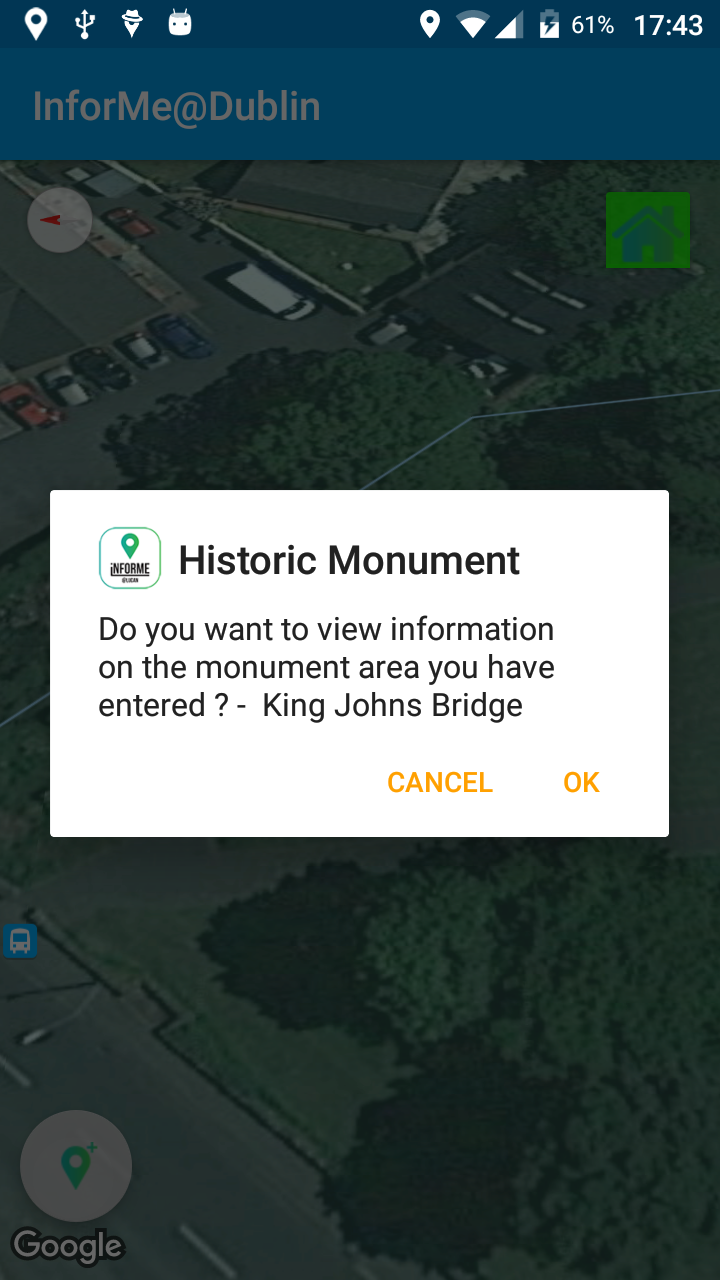
\includegraphics[width=150pt]{Geofence-Enter}
		\caption{Geofence Enter}
		\label{Figure: Geofence Enter}
	\end{minipage}
	\hfill
	\begin{minipage}[b]{0.4\textwidth}
		\includegraphics[width=150pt]{Information-Page}
		\caption{Information Page} 
		\label{Figure: Information Page}
	\end{minipage}
\end{figure}

\begin{figure}[!tbp]
	\centering
	\begin{minipage}[b]{0.4\textwidth}
		\includegraphics[width=150pt]{Display-Posts}
		\caption{Display Posts}
		\label{Figure: Display Posts}
	\end{minipage}
	\hfill
	\begin{minipage}[b]{0.4\textwidth}
		\includegraphics[width=150pt]{onClickPost}
		\caption{Entering Post} 
		\label{Figure: Entering Post}
	\end{minipage}
\end{figure}
%%%%%%%%%%%%%%%%%%%%%%%%%%%%%%%%%%%%%%%%%%%%%%%%%%%%%%%%%%%%%%%%%%5
\begin{figure}[!tbp]
	\centering
	\begin{minipage}[b]{0.4\textwidth}
		\includegraphics[width=150pt]{Adding-Geofence-Request-Email}
		\caption{Adding Geofence }
		\label{Figure: Adding Geofence}
	\end{minipage}
	\hfill
	\begin{minipage}[b]{0.4\textwidth}
		\includegraphics[width=150pt]{Add-Post}
		\caption{Add Post} 
		\label{Figure: Add Post}
	\end{minipage}
\end{figure}

\begin{figure}[!tbp]
	\centering
	\begin{minipage}[b]{0.4\textwidth}
		\includegraphics[width=150pt]{Updating-Post}
		\caption{ Updating Post}
		\label{Figure: Updating Post}
	\end{minipage}
	\hfill
	\begin{minipage}[b]{0.4\textwidth}
		\includegraphics[width=150pt]{onClickPost}
		\caption{Entering Post} 
		\label{Figure: Entering Post}
	\end{minipage}
\end{figure}
\chapter{Appendix B}

\section{InforMe@Dublin Code Listings}
In the following section of the appendices, the developer has submitted the code on which the InforMe@Dublin application was developed each section is split into its specific packages which are only related to its section such as Logging into the app, SettingsPreferences, Map\&Geofencing and also adding posts on a monument in the area. 

\section{Login\&Register}

\subsection{EmailPasswordAuthentication}

\lstinputlisting[language={Java},style=myCustomMatlabStyle, basicstyle=\small, breaklines, caption=EmailPasswordAuthentication,captionpos=b]{Email&Authenticatio.txt}

\subsection{Progress}

\lstinputlisting[language={Java},style=myCustomMatlabStyle, basicstyle=\small, breaklines, caption=Progress,captionpos=b]{Progress.txt}

\subsection{RegisterAccount}

\lstinputlisting[language={Java},style=myCustomMatlabStyle, basicstyle=\small, breaklines, caption=RegisterAccount,captionpos=b]{RegisterAccount.txt}

\subsection{SetupActivity}

\lstinputlisting[language={Java},style=myCustomMatlabStyle, basicstyle=\small, breaklines, caption=SetupActivity,captionpos=b]{SetupActivity.txt}

\subsection{ResetActivity}

\lstinputlisting[language={Java},style=myCustomMatlabStyle, basicstyle=\small, breaklines, caption=ResetActivity,captionpos=b]{ResetActivity.txt}

\section{Maps\&Geofencing}

\subsection{AddInformation}

\lstinputlisting[language={Java},style=myCustomMatlabStyle, basicstyle=\small, breaklines, caption=AddInformation,captionpos=b]{AddInformation.txt}

\subsection{Constants}

\lstinputlisting[language={Java},style=myCustomMatlabStyle, basicstyle=\small, breaklines, caption=Constants,captionpos=b]{Constants.txt}

\subsection{GeofenceTransitionsIntentService}

\lstinputlisting[language={Java},style=myCustomMatlabStyle, basicstyle=\small, breaklines, caption=GeofenceTransitionsIntentService,captionpos=b]{GeofenceTransitionsIntentService.txt}

\subsection{MapsActivity}

\lstinputlisting[language={Java},style=myCustomMatlabStyle, basicstyle=\small, breaklines, caption=MapsActivity,captionpos=b]{MapsActivity.txt}

\subsection{Place}

\lstinputlisting[language={Java},style=myCustomMatlabStyle, basicstyle=\small, breaklines, caption=Place,captionpos=b]{Place.txt}

\section{PostingInformation\&Comments}

\subsection{Comments}

\lstinputlisting[language={Java},style=myCustomMatlabStyle, basicstyle=\small, breaklines, caption=Comments,captionpos=b]{Comments.txt}

\subsection{CommentsActivity}

\lstinputlisting[language={Java},style=myCustomMatlabStyle, basicstyle=\small, breaklines, caption=CommentsActivity,captionpos=b]{CommentsActivity.txt}

\subsection{InformationFlipActivity}

\lstinputlisting[language={Java},style=myCustomMatlabStyle, basicstyle=\small, breaklines, caption=InformationFlipActivity,captionpos=b]{InformationFlipActivity.txt}

\subsection{InformationFrontFragment}

\lstinputlisting[language={Java},style=myCustomMatlabStyle, basicstyle=\small, breaklines, caption=InformationFrontFragment,captionpos=b]{InformationFrontFragment.txt}

\subsection{InformationBackCommentsFragment}

\lstinputlisting[language={Java},style=myCustomMatlabStyle, basicstyle=\small, breaklines, caption=InformationBackCommentsFragment,captionpos=b]{InformationBackCommentsFragment.txt}

\subsection{PostActivity}

\lstinputlisting[language={Java},style=myCustomMatlabStyle, basicstyle=\small, breaklines, caption=PostActivity,captionpos=b]{PostActivity.txt}

\subsection{UpdateActivity}

\lstinputlisting[language={Java},style=myCustomMatlabStyle, basicstyle=\small, breaklines, caption=UpdateActivity,captionpos=b]{UpdateActivity.txt}

\section{Settings}

\subsection{AppCompatPreferenceActivity}

\lstinputlisting[language={Java},style=myCustomMatlabStyle, basicstyle=\small, breaklines, caption=AppCompatPreferenceActivity,captionpos=b]{AppCompatPreferenceActivity.txt}

\subsection{SettingsActivity}

\lstinputlisting[language={Java},style=myCustomMatlabStyle, basicstyle=\small, breaklines, caption=SettingsActivity,captionpos=b]{SettingsActivity.txt}

\subsection{CheckConnectivity}

\lstinputlisting[language={Java},style=myCustomMatlabStyle, basicstyle=\small, breaklines, caption=CheckConnectivity,captionpos=b]{CheckConnectivity.txt}
\chapter{Appendix C}

\section{AndroidManifest}

\lstinputlisting[language={XML},style=myCustomMatlabStyle, basicstyle=\small, breaklines, caption= AndroidManifest,captionpos=b]{AndroidManifest.txt}

\chapter{Appendix D}

\section{Google-services.json}

\lstinputlisting[language={xml},style=myCustomMatlabStyle, basicstyle=\small, breaklines, caption= google-services,captionpos=b]{google-services.txt}

\setlinespacing{1.0}
\bibliographystyle{plainnat}
\bibliography{bibliography}

\end{document}
% ------------------------------------------------------------------------
%%%      \setlength\LTleft{1pt}
